%
% This document contains the chapter about linear and non-linear devices.
%
% Copyright (C) 2003, 2004, 2005, 2006, 2007 Stefan Jahn <stefan@lkcc.org>
% Copyright (C) 2003, 2004, 2005, 2006
%               Michael Margraf <Michael.Margraf@alumni.TU-Berlin.DE>
%
% Permission is granted to copy, distribute and/or modify this document
% under the terms of the GNU Free Documentation License, Version 1.1
% or any later version published by the Free Software Foundation.
%


\chapter{Non-linear devices}
%\addcontentsline{toc}{chapter}{Non-linear devices}
\label{sec:NLdevices}


\section{Operational amplifier}

The ideal operational amplifier, as shown in fig. \ref{fig:opamp}, is
determined by the following equation which introduces one more unknown
in the MNA matrix.

\begin{figure}[ht]
\begin{center}
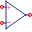
\includegraphics[width=4cm]{opamp}
\end{center}
\caption{ideal operational amplifier}
\label{fig:opamp}
\end{figure}
\FloatBarrier

\begin{equation}
V_{1} - V_{3} = 0
\label{eq:opamp}
\end{equation}

The new unknown variable $I_{out}$ must be considered by the three
remaining simple equations.

\begin{equation}
I_{1} = 0 \quad I_{2} = I_{out} \quad I_{3} = 0
\end{equation}

And in matrix representation this is (for DC and AC simulation):
\begin{equation}
\begin{bmatrix}
.&.&.& 0\\
.&.&.& 1\\
.&.&.& 0\\
1 & 0 & -1 & 0
\end{bmatrix}
\cdot
\begin{bmatrix}
V_{1}\\
V_{2}\\
V_{3}\\
I_{out}
\end{bmatrix}
=
\begin{bmatrix}
I_{1}\\
I_{2}\\
I_{3}\\
0
\end{bmatrix}
\end{equation}

The operational amplifier could be considered as a special case of a
voltage controlled current source with infinite forward
transconductance $G$.  Please note that the presented matrix form is
only valid in cases where there is a finite feedback impedance
between the output and the inverting input port.

\addvspace{12pt}

To allow a feedback circuit to the non-inverting input (e.g.  for a
Schmitt trigger), one needs a limited output voltage swing.  The
following equations are often used to model the transmission
characteristic of operational amplifiers.
\begin{equation}
I_1 = 0 \qquad\qquad I_3 = 0
\end{equation}
\begin{equation}
\label{eq:OPVout}
V_2 = V_{max}\cdot\dfrac{2}{\pi}\arctan \left( \dfrac{\pi}{2\cdot V_{max}}\cdot G\cdot (V_1-V_3) \right)
\end{equation}

with $V_{max}$ being the maximum output voltage swing and $G$ the
voltage amplification.  To model the small-signal behaviour (AC
analysis), it is necessary to differentiate:
\begin{equation}
g = \dfrac{\partial V_2}{\partial (V_1-V_3)}
  = \dfrac{G}{1+\left( \dfrac{\pi}{2\cdot V_{max}}\cdot G\cdot (V_1-V_3) \right)^2}
\end{equation}

This leads to the following matrix representation being a specialised
three node voltage controlled voltage source (see section
\ref{sec:vcvs} on page \pageref{sec:vcvs}).
\begin{equation}
\begin{bmatrix}
.&.&.& 0\\
.&.&.& 1\\
.&.&.& 0\\
g & -1 & -g & 0
\end{bmatrix}
\cdot
\begin{bmatrix}
V_{1}\\
V_{2}\\
V_{3}\\
I_{out}
\end{bmatrix}
=
\begin{bmatrix}
I_{1}\\
I_{2}\\
I_{3}\\
0
\end{bmatrix}
\end{equation}

The above MNA matrix entries are also used during the non-linear DC
analysis with the 0 in the right hand side vector replaced by an
equivalent voltage
\begin{equation}
V_{eq} = g\cdot \left(V_1 - V_3\right) - V_{out}
\end{equation}
with $V_{out}$ computed using eq. \eqref{eq:OPVout}.

\addvspace{12pt}

With the given small-signal matrix representation, building the
S-parameters is easy.
\begin{equation}
(\underline{S}) =
\begin{bmatrix}
 1  &  0 & 0  \\
 4g & -1 & -4g\\
 0  &  0 &  1
\end{bmatrix}
\end{equation}


\section{PN-Junction Diode}
%\addcontentsline{toc}{section}{PN-Junction Diode}

The following table contains the model parameters for the pn-junction
diode model.

\addvspace{12pt}

\begin{longtable}{rllll}
Name & Symbol & Description & Unit & Default\\
\hline
\endhead
Is & $I_{S}$ & saturation current & $\ampere$ & $10^{-14}$\\
N & $N$ & emission coefficient & & $1.0$\\
Isr & $I_{SR}$ & recombination current parameter & $\ampere$ & $0.0$\\
Nr & $N_{R}$ & emission coefficient for Isr & & $2.0$\\
Rs & $R_{S}$ & ohmic resistance & $\ohm$ & $0.0$\\
Cj0 & $C_{j0}$ & zero-bias junction capacitance & $\farad$ & $0.0$\\
M & $M$ & grading coefficient & & $0.5$\\
Vj & $V_{j}$ & junction potential & $\volt$ & $0.7$\\
Fc & $F_{c}$ & forward-bias depletion capacitance coefficient & & $0.5$\\
Cp & $C_{p}$ & linear capacitance & $\farad$ & $0.0$\\
Tt & $\tau$ & transit time & $\second$ & $0.0$\\
Bv & $B_v$ & reverse breakdown voltage & $\volt$ & $\infty$\\
Ibv & $I_{Bv}$ & current at reverse breakdown voltage & $\ampere$ & $0.001$\\
Kf & $K_F$ & flicker noise coefficient & & $0.0$\\
Af & $A_F$ & flicker noise exponent & & $1.0$\\
Ffe & $F_{FE}$ & flicker noise frequency exponent & & $1.0$\\
Temp & $T$ & device temperature & $\degree \mathrm{C}$ & $26.85$\\
Xti & $X_{TI}$ & saturation current exponent & & $3.0$\\
Eg & $E_G$ & energy bandgap & eV & $1.11$\\
Tbv & $T_{Bv}$ & Bv linear temperature coefficient & $1/\degree \mathrm{C}$ & $0.0$\\
Trs & $T_{RS}$ & Rs linear temperature coefficient & $1/\degree \mathrm{C}$ & $0.0$\\
Ttt1 & $T_{\tau 1}$ & Tt linear temperature coefficient & $1/\degree \mathrm{C}$ & $0.0$\\
Ttt2 & $T_{\tau 2}$ & Tt quadratic temperature coefficient & $1/\degree \mathrm{C}^2$ & $0.0$\\
Tm1 & $T_{M1}$ & M linear temperature coefficient & $1/\degree \mathrm{C}$ & $0.0$\\
Tm2 & $T_{M2}$ & M quadratic temperature coefficient & $1/\degree \mathrm{C}^2$ & $0.0$\\
Tnom & $T_{NOM}$ & temperature at which parameters were extracted & $\degree \mathrm{C}$ & $26.85$\\
Area & $A$ & default area for diode & & $1.0$
\end{longtable}

\addvspace{12pt}

\subsection{Large signal model}
%\addcontentsline{toc}{subsection}{Large signal model}

\begin{figure}[ht]
\begin{center}
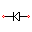
\includegraphics[width=0.3\linewidth]{diode}
\end{center}
\caption{pn-junction diode symbol and large signal model}
\label{fig:diode}
\end{figure}
\FloatBarrier

The current equation of the diode and its derivative writes as
follows:
\begin{align}
I_{d} &= I_{S}\cdot \left(e^{\frac{V_{d}}{N\cdot V_{T}}} - 1\right) + I_{SR}\cdot \left(e^{\frac{V_{d}}{N_R\cdot V_{T}}} - 1\right)\\
g_{d} &= \dfrac{\partial I_{d}}{\partial V_{d}} = \dfrac{I_{S}}{N\cdot V_{T}}\cdot e^{\frac{V_{d}}{N\cdot V_{T}}} + \dfrac{I_{SR}}{N_R\cdot V_{T}}\cdot e^{\frac{V_{d}}{N_R\cdot V_{T}}}
\end{align}

\begin{figure}[ht]
\begin{center}
\includegraphics[width=0.17\linewidth]{dcdiode}
\end{center}
\caption{accompanied DC model of intrinsic diode}
\label{fig:dcdiode}
\end{figure}
\FloatBarrier

The complete MNA matrix entries are:
\begin{equation}
\begin{bmatrix}
g_{d} & -g_{d}\\
-g_{d} & g_{d}\\
\end{bmatrix}
\cdot
\begin{bmatrix}
V_{C}\\
V_{A}\\
\end{bmatrix}
=
\begin{bmatrix}
+I_{d} - g_{d}\cdot V_{d}\\
-I_{d} + g_{d}\cdot V_{d}\\
\end{bmatrix}
\end{equation}

\subsection{Small signal model}
%\addcontentsline{toc}{subsection}{Small signal model}

\begin{figure}[ht]
\begin{center}
\includegraphics[width=0.17\linewidth]{spdiode}
\end{center}
\caption{small signal model of intrinsic diode}
\label{fig:spdiode}
\end{figure}
\FloatBarrier

The voltage dependent capacitance consists of a diffusion capacitance,
a junction capacitance and an additional linear capacitance which is
usually modeled by the following equations.

\begin{equation}
C_{d} = C_p + \tau \cdot g_{d} +
\begin{cases}
\begin{array}{ll}
C_{j0}\cdot \left(1 - \dfrac{V_{d}}{V_{j}}\right)^{-M} & \textrm{ for } V_{d} \le F_c\cdot V_j\\
\dfrac{C_{j0}}{\left(1 - F_c\right)^M}\cdot \left(1 + \dfrac{M\cdot \left(V_{d} - F_c\cdot V_j\right)}{V_{j}\cdot\left(1 - F_c\right)}\right) & \textrm{ for } V_{d} > F_c\cdot V_j
\end{array}
\end{cases}
\end{equation}

The S-parameters of the passive circuit shown in
fig. \ref{fig:spdiode} can be written as
\begin{align}
S_{11} = S_{22} &= \dfrac{1}{1 + 2\cdot y}\\
S_{12} = S_{21} &= 1 - S_{11} = \dfrac{2\cdot y}{1 + 2\cdot y}
\end{align}

with
\begin{equation}
y = Z_{0}\cdot \left(g_{d} + j\omega C_{d}\right)
\end{equation}

\subsection{Noise model}
%\addcontentsline{toc}{subsection}{Noise model}
\label{sec:nw_diode}

The thermal noise generated by the series resistor is characterized by
the following spectral density.
\begin{equation}
\dfrac{\overline{i_{R_S}^2}}{\Delta f} = \dfrac{4 k_B T}{R_S}
\end{equation}

\begin{figure}[ht]
\begin{center}
\includegraphics[width=0.28\linewidth]{noisediode}
\end{center}
\caption{noise model of intrinsic diode}
\label{fig:noisediode}
\end{figure}
\FloatBarrier

The shot noise and flicker noise generated by the DC current flow
through the diode is characterized by the following spectral density.
\begin{equation}
\dfrac{\overline{i_{d}^2}}{\Delta f} = 2e I_d + K_F \dfrac{I_d^{A_F}}{f^{F_{FE}}}
\end{equation}

Thus the noise current correlation matrix can be formed.  This matrix
can be easily converted to the noise wave correlation matrix
representation using the formulas given in section
\ref{sec:noiseTrans} on page \pageref{sec:noiseTrans}.
\begin{equation}
\underline{C}_Y = \Delta f
\begin{bmatrix}
+\overline{i_{d}^2} & -\overline{i_{d}^2}\\
-\overline{i_{d}^2} & +\overline{i_{d}^2}\\
\end{bmatrix}
\end{equation}

An ideal diode (pn- or schottky-diode) generates shot noise.  Both
types of current (field and diffusion) contribute independently to it.
That is, even though the two currents flow in different directions
("minus" in dc current equation), they have to be added in the noise
equation (current is proportional to noise power spectral density).
Taking into account the dynamic conductance $g_d$ in parallel to the
noise current source, the noise wave correlation matrix writes as
follows.

\begin{equation}
\begin{split}
(\underline{C})
 =  \left| \frac{0.5\cdot Y_0}{g_d+j\omega C_d + 0.5\cdot Y_0}\right|^2  \cdot 2\cdot e\cdot I_S\cdot
    \left( \exp\left( \frac{V_{d}}{N\cdot V_T} \right) +1 \right) \cdot Z_0\cdot\begin{pmatrix}
   1 & -1\\
  -1 &  1\\
\end{pmatrix} \\
 = 2\cdot e\cdot Z_0\cdot \left(I_{d} + 2\cdot I_{S}\right)\cdot
    \left| \frac{1}{2\cdot Z_0\cdot (g_d+j\omega C_d) + 1}\right|^2 \cdot
\begin{pmatrix}
   1 & -1\\
  -1 &  1\\
\end{pmatrix}
\end{split}
\end{equation}

Where $e$ is charge of an electron, $V_T$ the temperature voltage,
$g_d$ the (dynamic) conductance of the diode and $C_d$ its junction
capacitance.

\addvspace{12pt}

To be very precise, the equation above only holds for diodes whose
field and diffusion current dominate absolutely (diffusion limited
diode), i.e. $N=1$.  Many diodes also generate a
generation/recombination current ($N\approx 2$), which produces shot
noise, too.  But depending on where and how the charge carriers
generate or recombine, their effective charge is somewhat smaller than
$e$.  To take this into account, one needs a further factor $K$.
Several opinions exist according the value of $K$.  Some say 1 and 2/3
are common values, others say $K=1/N$ with $K$ and $N$ being bias
dependent.  Altogether it is:
\begin{equation}
\begin{split}
(\underline{C})
 = 2\cdot e\cdot Z_0\cdot K\cdot \left(I_{d} + 2\cdot I_{S}\right)\cdot
    \left| \frac{1}{2\cdot Z_0\cdot (g_d+j\omega C_d) + 1}\right|^2 \cdot
\begin{pmatrix}
   1 & -1\\
  -1 &  1\\
\end{pmatrix}\\
\text{with}\qquad\frac{1}{2}\le K \le 1
\end{split}
\label{eq:diode_noise}
\end{equation}

Remark: Believing the diode equation $I_D = I_S\cdot (\exp(V/(N\cdot
V_T)) - 1)$ is the whole truth, it is logical to define $K=1/N$,
because at $V=0$ the conductance $g_d$ of the diode must create
thermal noise.

\addvspace{12pt}

Some special diodes have additional current or noise components
(tunnel diodes, avalanche diodes etc.).  All these mechanisms are not
taken into account in equation \eqref{eq:diode_noise}.

\addvspace{12pt}

The parasitic ohmic resistance in a non-ideal diode, of course,
creates thermal noise.

Noise current correlation matrix (for details on the parameters
see above):
\begin{equation}
(\underline{C}_Y)
 = 2\cdot e\cdot K\cdot \left(I_{d} + 2\cdot I_{S}\right)\cdot
\begin{pmatrix}
   1 & -1\\
  -1 &  1\\
\end{pmatrix}\\
\end{equation}


\subsection{Temperature model}
%\addcontentsline{toc}{subsection}{Temperature model}
\label{sec:DiodeTemp}

This section mathematically describes the dependencies of the diode
characterictics on temperature.  For a junction diode a typical value
for $X_{TI}$ is $3.0$, for a Schottky barrier diode it is $2.0$.  The
energy band gap at zero temperature $E_G$ is by default $1.11$eV.  For
other materials than Si, $0.69$eV (for a Schottky barrier diode),
$0.67$eV (for Ge) and $1.43$eV (for GaAs) should be used.
\begin{align}
n_i^2\left(T\right) &= B\cdot T^3 \cdot e^{-E_G\left(T\right)/k_B T}\\
n_i\left(T\right) &= 1.45\cdot 10^{10}\cdot \left(\dfrac{T}{300K}\right)^{1.5}\cdot\exp{\left(\dfrac{e\cdot E_G\left(300K\right)}{2\cdot k_B\cdot 300K} - \dfrac{e\cdot E_G\left(T\right)}{2\cdot k_B\cdot T}\right)}\\
E_G\left(T\right) &= E_G - \dfrac{\alpha\cdot T^2}{\beta + T}
\end{align}

with experimental values for Si given by
\begin{align*}
\alpha &= 7.02\cdot 10^{-4}\\
\beta &= 1108\\
E_G &= 1.16eV
\end{align*}

The following equations show the temperature dependencies of the diode
parameters.  The reference temperature $T_1$ in these equations
denotes the nominal temperature $T_{NOM}$ specified by the diode
model.
\begin{align}
I_S\left(T_2\right) &= I_S\left(T_1\right)\cdot \left(\dfrac{T_2}{T_1}\right)^{X_{TI} / N} \cdot \exp{\left[-\dfrac{e\cdot E_G\left(300K\right)}{N\cdot k_B\cdot T_2}\cdot \left(1 - \dfrac{T_2}{T_1}\right)\right]}\\
V_j\left(T_2\right) &= \dfrac{T_2}{T_1}\cdot V_j\left(T_1\right) + \dfrac{2\cdot k_B\cdot T_2}{e} \cdot \ln{\left(\dfrac{n_i\left(T_1\right)}{n_i\left(T_2\right)}\right)}\\
 &= \dfrac{T_2}{T_1}\cdot V_j\left(T_1\right) - \dfrac{2\cdot k_B\cdot T_2}{e} \cdot \ln{\left(\dfrac{T_2}{T_1}\right)^{1.5}} - \left(\dfrac{T_2}{T_1} \cdot E_G\left(T_1\right) - E_G\left(T_2\right)\right)\\
C_{j0}\left(T_2\right) &= C_{j0}\left(T_1\right)\cdot\left(1 + M\cdot\left(400\cdot 10^{-6} \cdot\left(T_2 - T_1\right) - \dfrac{V_j\left(T_2\right) - V_j\left(T_1\right)}{V_j\left(T_1\right)}\right)\right)
\end{align}

Some additionial temperature coefficients determine the temperature
dependence of even more model parameters.
\begin{align}
B_{v}\left(T_2\right) &= B_{v}\left(T_1\right) - T_{Bv}\cdot\left(T_2 - T_1\right)\\
\tau\left(T_2\right) &= \tau\left(T_1\right)\cdot\left(1 + T_{\tau 1}\cdot\left(T_2 - T_1\right) + T_{\tau 2}\cdot\left(T_2 - T_1\right)^2\right)\\
M\left(T_2\right) &= M\left(T_1\right)\cdot\left(1 + T_{M1}\cdot\left(T_2 - T_1\right) + T_{M2}\cdot\left(T_2 - T_1\right)^2\right)\\
R_S\left(T_2\right) &= R_S\left(T_1\right)\cdot\left(1 + T_{RS}\cdot\left(T_2 - T_1\right)\right)
\end{align}

\subsection{Area dependence of the model}
%\addcontentsline{toc}{subsection}{Area dependence of the model}

The area factor $A$ used in the diode model determines the number of
equivalent parallel devices of the specified model.  The diode model
parameters affected by the $A$ factor are:
\begin{align}
I_S\left(A\right) &= I_S\cdot A\\
C_{j0}\left(A\right) &= C_{j0}\cdot A\\
R_S\left(A\right) &= \dfrac{R_S}{A}
\end{align}

\section{Junction FET}
%\addcontentsline{toc}{section}{Junction FET}

The following table contains the model parameters for the JFET model.

\addvspace{12pt}

\begin{longtable}{rllll}
Name & Symbol & Description & Unit & Default\\
\hline
\endhead
Vt0 & $V_{Th}$ & zero -bias threshold voltage & $\volt$ & $-2.0$\\
Beta & $\beta$ & transconductance parameter & $\ampere / \volt^{2}$ & $10^{-4}$\\
Lambda & $\lambda$ & channel-length modulation parameter & $1/\volt$ & $0.0$\\
Rd & $R_{D}$ & drain ohmic resistance & $\ohm$ & $0.0$\\
Rs & $R_{S}$ & source ohmic resistance & $\ohm$ & $0.0$\\
Is & $I_{S}$ & gate-junction saturation current & $\ampere$ & $10^{-14}$\\
N & $N$ & gate P-N emission coefficient & & $1.0$\\
Isr & $I_{SR}$ & gate-junction recombination current parameter & $\ampere$ & $0.0$\\
Nr & $N_{R}$ & Isr emission coefficient & & $2.0$\\
Cgs & $C_{gs}$ & zero-bias gate-source junction capacitance & $\farad$ & $0.0$\\
Cgd & $C_{gd}$ & zero-bias gate-drain junction capacitance & $\farad$ & $0.0$\\
Pb & $P_{b}$ & gate-junction potential & $\volt$ & $1.0$\\
Fc & $F_{c}$ & forward-bias junction capacitance coefficient & & $0.5$\\
M & $M$ & gate P-N grading coefficient & & $0.5$\\
Kf & $K_F$ & flicker noise coefficient & & $0.0$\\
Af & $A_F$ & flicker noise exponent & & $1.0$\\
Ffe & $F_{FE}$ & flicker noise frequency exponent & & $1.0$\\
Temp & $T$ & device temperature & $\degree \mathrm{C}$ & $26.85$\\
Xti & $X_{TI}$ & saturation current exponent & & $3.0$\\
Vt0tc & $V_{Th_{TC}}$ & Vt0 temperature coefficient & $\volt/\degree \mathrm{C}$ & $0.0$\\
Betatce & $\beta_{TCE}$ & Beta exponential temperature coefficient & $\%/\degree \mathrm{C}$ & $0.0$\\
Tnom & $T_{NOM}$ & temperature at which parameters were extracted & $\degree \mathrm{C}$ & $26.85$\\
Area & $A$ & default area for JFET & & $1.0$
\end{longtable}

\addvspace{12pt}

\subsection{Large signal model}
%\addcontentsline{toc}{subsection}{Large signal model}

\begin{figure}[ht]
\begin{center}
\includegraphics[width=0.5\linewidth]{jfet}
\end{center}
\caption{junction FET symbol and large signal model}
\label{fig:jfet}
\end{figure}
\FloatBarrier

The current equation of the gate source diode and its derivative
writes as follows:
\begin{align}
I_{GS} &= I_{S}\cdot \left(e^{\frac{V_{GS}}{N\cdot V_{T}}} - 1\right) + I_{SR}\cdot \left(e^{\frac{V_{GS}}{N_{R}\cdot V_{T}}} - 1\right)\\
g_{gs} &= \dfrac{\partial I_{GS}}{\partial V_{GS}} = \dfrac{I_{S}}{N\cdot V_{T}}\cdot e^{\frac{V_{GS}}{N\cdot V_{T}}} + \dfrac{I_{SR}}{N_{R}\cdot V_{T}}\cdot e^{\frac{V_{GS}}{N_{R}\cdot V_{T}}}
\end{align}

The current equation of the gate drain diode and its derivative writes
as follows:
\begin{align}
I_{GD} &= I_{S}\cdot \left(e^{\frac{V_{GD}}{N\cdot V_{T}}} - 1\right) + I_{SR}\cdot \left(e^{\frac{V_{GD}}{N_{R}\cdot V_{T}}} - 1\right)\\
g_{gd} &= \dfrac{\partial I_{GD}}{\partial V_{GD}} = \dfrac{I_{S}}{N\cdot V_{T}}\cdot e^{\frac{V_{GD}}{N\cdot V_{T}}} + \dfrac{I_{SR}}{N_{R}\cdot V_{T}}\cdot e^{\frac{V_{GD}}{N_{R}\cdot V_{T}}}
\end{align}

Both equations contain the gate-junction saturation current $I_{S}$,
the gate P-N emission coefficient $N$ and the temperature voltage
$V_{T}$ with the Boltzmann's constant $k_{B}$ and the electron charge
$q$.  The operating temperature $T$ must be specified in Kelvin.
\begin{equation}
V_{T} = \dfrac{k_{B}\cdot T}{q}
\end{equation}

The controlled drain currents have been defined by Shichman and Hodges
\cite{Shichman} for different modes of operations.

\begin{equation}
g_{m} = \dfrac{\partial I_{d}}{\partial V_{GS}}
\;\;\;\; \text{ and } \;\;\;\;
g_{ds} = \dfrac{\partial I_{d}}{\partial V_{DS}}
\;\;\;\; \text{ with } \;\;\;\;
V_{GD} = V_{GS} - V_{DS}
\end{equation}

\begin{itemize}
\item normal mode: $V_{DS} > 0$
\begin{itemize}
\item normal mode, cutoff region: $V_{GS} - V_{Th} < 0$
\begin{align}
I_{d} &= 0\\
g_{m} &= 0\\
g_{ds} &= 0\\
%\end{align}
\intertext{
\item normal mode, saturation region: $0 < V_{GS} - V_{Th} < V_{DS}$
}
%\begin{align}
I_{d} &= \beta \cdot\left(1 + \lambda V_{DS}\right) \cdot\left(V_{GS} - V_{Th}\right)^{2}\\
g_{m} &= \beta \cdot\left(1 + \lambda V_{DS}\right) \cdot 2\left(V_{GS} - V_{Th}\right)\\
g_{ds} &= \beta \cdot \lambda\left(V_{GS} - V_{Th}\right)^{2}\\
%\end{align}
\intertext{
\item normal mode, linear region: $V_{DS} < V_{GS} - V_{Th}$
}
%\begin{align}
I_{d} &= \beta\cdot\left(1 + \lambda V_{DS}\right)\cdot\left(2 \left(V_{GS} - V_{Th}\right) - V_{DS}\right)\cdot V_{DS}\\
g_{m} &= \beta\cdot\left(1 + \lambda V_{DS}\right)\cdot 2\cdot V_{DS}\\
g_{ds} &= \beta\cdot\left(1 + \lambda V_{DS}\right)\cdot 2\left(V_{GS} - V_{Th} - V_{DS}\right) + \beta \cdot \lambda V_{DS}\cdot\left(2\left(V_{GS} - V_{Th}\right) - V_{DS}\right)
\end{align}
\end{itemize}
\item inverse mode: $V_{DS} < 0$
\begin{itemize}
\item inverse mode, cutoff region: $V_{GD} - V_{Th} < 0$
\begin{align}
I_{d} &= 0\\
g_{m} &= 0\\
g_{ds} &= 0\\
%\end{align}
\intertext{
\item inverse mode, saturation region: $0 < V_{GD} - V_{Th} < -V_{DS}$
}
%\begin{align}
I_{d} &= -\beta \cdot\left(1 - \lambda V_{DS}\right) \cdot\left(V_{GD} - V_{Th}\right)^{2}\\
g_{m} &= -\beta \cdot\left(1 - \lambda V_{DS}\right) \cdot 2\left(V_{GD} - V_{Th}\right)\\
g_{ds} &= \beta \cdot\lambda \left(V_{GD} - V_{Th}\right)^{2} + \beta\cdot\left(1 - \lambda V_{DS}\right) \cdot 2\left(V_{GD} - V_{Th}\right)\\
%\end{align}
\intertext{
\item inverse mode, linear region: $-V_{DS} < V_{GD} - V_{Th}$
}
%\begin{align}
I_{d} &= \beta\cdot\left(1 - \lambda V_{DS}\right)\cdot\left(2 \left(V_{GD} - V_{Th}\right) + V_{DS}\right)\cdot V_{DS}\\
g_{m} &= \beta\cdot\left(1 - \lambda V_{DS}\right)\cdot 2\cdot V_{DS}\\
g_{ds} &= \beta\cdot\left(1 - \lambda V_{DS}\right)\cdot 2\left(V_{GD} - V_{Th}\right) - \beta \cdot \lambda V_{DS}\cdot\left(2\left(V_{GD} - V_{Th}\right) + V_{DS}\right)
\end{align}
\end{itemize}
\end{itemize}

The MNA matrix entries for the voltage controlled drain current source
can be written as:

\addvspace{12pt}

\begin{center}
\begin{tabular}{p{1.5cm}|lll}
\raggedleft & \centering G & \centering S & controlling nodes\\
\hline
\raggedleft D & $+g_{m}$ & $-g_{m}$ &\\
\raggedleft S & $-g_{m}$ & $+g_{m}$ &\\
\raggedleft controlled nodes & & &
\end{tabular}
\end{center}

\addvspace{12pt}

With the accompanied DC model shown in fig. \ref{fig:dcjfet} using the
same principles as explained in section \ref{sec:DCdiode} on page
\pageref{sec:DCdiode} it is possible to build the complete MNA matrix
of the intrinsic JFET.

\begin{figure}[ht]
\begin{center}
\includegraphics[width=0.5\linewidth]{dcjfet}
\end{center}
\caption{accompanied DC model of intrinsic JFET}
\label{fig:dcjfet}
\end{figure}
\FloatBarrier

Applying the rules for creating the MNA matrix of an arbitrary network
the complete MNA matrix entries (admittance matrix and current vector)
for the intrinsic junction FET are:
\begin{equation}
\begin{bmatrix}
g_{gd} + g_{gs} & -g_{gd} & -g_{gs}\\
-g_{gd} + g_{m} & g_{ds} + g_{gd} & -g_{ds} - g_{m}\\
-g_{gs} - g_{m} & -g_{ds} & g_{gs} + g_{ds} + g_{m}
\end{bmatrix}
\cdot
\begin{bmatrix}
V_{G}\\
V_{D}\\
V_{S}\\
\end{bmatrix}
=
\begin{bmatrix}
-I_{GD_{eq}} - I_{GS_{eq}}\\
+I_{GD_{eq}} - I_{DS_{eq}}\\
+I_{GS_{eq}} + I_{DS_{eq}}
\end{bmatrix}
\end{equation}

with
\begin{align}
I_{GS_{eq}} &= I_{GS} - g_{gs}\cdot V_{GS}\\
I_{GD_{eq}} &= I_{GD} - g_{gd}\cdot V_{GD}\\
I_{DS_{eq}} &= I_{d} - g_{m}\cdot V_{GS} - g_{ds}\cdot V_{DS}
\end{align}

\subsection{Small signal model}
%\addcontentsline{toc}{subsection}{Small signal model}

\begin{figure}[ht]
\begin{center}
\includegraphics[width=0.45\linewidth]{spjfet}
\end{center}
\caption{small signal model of intrinsic junction FET}
\label{fig:spjfet}
\end{figure}
\FloatBarrier

The small signal Y-parameter matrix of the intrinsic junction FET
writes as follows.  It can be converted to S-parameters.
\begin{equation}
Y =
\begin{bmatrix}
Y_{GD} + Y_{GS} & -Y_{GD} & -Y_{GS}\\
g_{m} - Y_{GD} & Y_{GD} + Y_{DS} & -Y_{DS} - g_{m}\\
-g_{m} - Y_{GS} & -Y_{DS} & Y_{GS} + Y_{DS} + g_{m}\\
\end{bmatrix}
\end{equation}

with
\begin{align}
Y_{GD} &= g_{gd} + j\omega C_{GD}\\
Y_{GS} &= g_{gs} + j\omega C_{GS}\\
Y_{DS} &= g_{ds}
\end{align}

The junction capacitances are modeled with the following equations.

\begin{align}
C_{GD} &= 
\begin{cases}
\begin{array}{ll}
C_{gd}\cdot \left(1 - \dfrac{V_{GD}}{P_{b}}\right)^{-M} & \textrm{ for } V_{GD} \le F_{c}\cdot P_{b}\\
\dfrac{C_{gd}}{\left(1 - F_{c}\right)^{M}}\cdot \left(1 + \dfrac{M\cdot \left(V_{GD} - F_{c}\cdot P_{b}\right)}{P_{b}\cdot \left(1 - F_{c}\right)}\right) & \textrm{ for } V_{GD} > F_{c}\cdot P_{b}
\end{array}
\end{cases}\\
C_{GS} &= 
\begin{cases}
\begin{array}{ll}
C_{gs}\cdot \left(1 - \dfrac{V_{GS}}{P_{b}}\right)^{-M} & \textrm{ for } V_{GS} \le F_{c}\cdot P_{b}\\
\dfrac{C_{gs}}{\left(1 - F_{c}\right)^{M}}\cdot \left(1 + \dfrac{M\cdot \left(V_{GS} - F_{c}\cdot P_{b}\right)}{P_{b}\cdot \left(1 - F_{c}\right)}\right) & \textrm{ for } V_{GS} > F_{c}\cdot P_{b}
\end{array}
\end{cases}
\end{align}

\subsection{Noise model}
%\addcontentsline{toc}{subsection}{Noise model}

Both the drain and source resistance $R_D$ and $R_S$ generate thermal
noise characterized by the following spectral density.
\begin{equation}
\dfrac{\overline{i_{R_D}^2}}{\Delta f} = \dfrac{4 k_B T}{R_D}
\;\;\;\; \textrm{ and } \;\;\;\;
\dfrac{\overline{i_{R_S}^2}}{\Delta f} = \dfrac{4 k_B T}{R_S}
\end{equation}

\begin{figure}[ht]
\begin{center}
\includegraphics[width=0.58\linewidth]{noisejfet}
\end{center}
\caption{noise model of intrinsic junction FET}
\label{fig:noisejfet}
\end{figure}
\FloatBarrier

Channel noise and flicker noise generated by the DC transconductance
$g_m$ and current flow from drain to source is characterized by the
following spectral density.
\begin{equation}
\dfrac{\overline{i_{ds}^2}}{\Delta f} = \dfrac{8 k_B T g_m}{3} + K_F\dfrac{I_{DS}^{A_F}}{f^{F_{FE}}}
\end{equation}

The noise current correlation matrix (admittance representation) of
the intrinsic junction FET can be expressed by
\begin{equation}
\underline{C}_Y = \Delta f
\begin{bmatrix}
0 & 0 & 0\\
0 & +\overline{i_{ds}^2} & -\overline{i_{ds}^2}\\
0 & -\overline{i_{ds}^2} & +\overline{i_{ds}^2}\\
\end{bmatrix}
\end{equation}

This matrix representation can be easily converted to the noise-wave
representation $\underline{C}_S$ if the small signal S-parameter
matrix is known.

\subsection{Temperature model}
%\addcontentsline{toc}{subsection}{Temperature model}

Temperature appears explicitly in the exponential terms of the JFET
model equations.  In addition, saturation current, gate-junction
potential and zero-bias junction capacitances have built-in
temperature dependence.
\begin{align}
I_S\left(T_2\right) &= I_S\left(T_1\right)\cdot \left(\dfrac{T_2}{T_1}\right)^{X_{TI} / N} \cdot \exp{\left[-\dfrac{e\cdot E_G\left(300K\right)}{N\cdot k_B\cdot T_2}\cdot \left(1 - \dfrac{T_2}{T_1}\right)\right]}\\
I_{SR}\left(T_2\right) &= I_{SR}\left(T_1\right)\cdot \left(\dfrac{T_2}{T_1}\right)^{X_{TI} / N_R} \cdot \exp{\left[-\dfrac{e\cdot E_G\left(300K\right)}{N_R\cdot k_B\cdot T_2}\cdot \left(1 - \dfrac{T_2}{T_1}\right)\right]}\\
P_{b}\left(T_2\right)  &= \dfrac{T_2}{T_1}\cdot P_{b}\left(T_1\right) - \dfrac{2\cdot k_B\cdot T_2}{e} \cdot \ln{\left(\dfrac{T_2}{T_1}\right)^{1.5}} - \left(\dfrac{T_2}{T_1} \cdot E_G\left(T_1\right) - E_G\left(T_2\right)\right)\\
C_{gs}\left(T_2\right) &= C_{gs}\left(T_1\right)\cdot\left(1 + M\cdot\left(400\cdot 10^{-6} \cdot\left(T_2 - T_1\right) - \dfrac{P_{b}\left(T_2\right) - P_{b}\left(T_1\right)}{P_{b}\left(T_1\right)}\right)\right)\\
C_{gd}\left(T_2\right) &= C_{gd}\left(T_1\right)\cdot\left(1 + M\cdot\left(400\cdot 10^{-6} \cdot\left(T_2 - T_1\right) - \dfrac{P_{b}\left(T_2\right) - P_{b}\left(T_1\right)}{P_{b}\left(T_1\right)}\right)\right)
\end{align}

where the $E_G\left(T\right)$ dependency has already been described in
section \ref{sec:DiodeTemp} on page \pageref{sec:DiodeTemp}.  Also the
threshold voltage as well as the transconductance parameter have a
temperature dependence determined by
\begin{align}
V_{Th}\left(T_2\right) &= V_{Th}\left(T_1\right) + V_{Th_{TC}}\cdot\left(T_2 - T_1\right)\\
\beta\left(T_2\right) &= \beta\left(T_1\right)\cdot 1.01^{\beta_{TCE}\cdot\left(T_2 - T_1\right)}
\end{align}

\subsection{Area dependence of the model}
%\addcontentsline{toc}{subsection}{Area dependence of the model}

The area factor $A$ used for the JFET model determines the number of
equivalent parallel devices of a specified model.  The following
parameters are affected by the area factor.
\begin{align}
\beta\left(A\right) &= \beta\cdot A & I_S\left(A\right) &= I_S\cdot A\\
R_D\left(A\right) &= \dfrac{R_D}{A} & R_S\left(A\right) &= \dfrac{R_S}{A}\\
C_{gs}\left(A\right) &= C_{gs}\cdot A & C_{gd}\left(A\right) &= C_{gd}\cdot A
\end{align}

\section{Homo-Junction Bipolar Transistor}
%\addcontentsline{toc}{section}{Bipolar Transistor}

The following table contains the model parameters for the BJT (Spice
Gummel-Poon) model.

\addvspace{12pt}

\begin{longtable}{rllll}
Name & Symbol & Description & Unit & Default\\
\hline
\endhead
Is & $I_{S}$ & saturation current & $\ampere$ & $10^{-16}$\\
Nf & $N_F$ & forward emission coefficient & & $1.0$\\
Nr & $N_R$ & reverse emission coefficient & & $1.0$\\
Ikf & $I_{KF}$ & high current corner for forward beta & $\ampere$ & $\infty$\\
Ikr & $I_{KR}$ & high current corner for reverse beta & $\ampere$ & $\infty$\\
Vaf & $V_{AF}$ & forward early voltage & $\volt$ & $\infty$\\
Var & $V_{AR}$ & reverse early voltage & $\volt$ & $\infty$\\
Ise & $I_{SE}$ & base-emitter leakage saturation current & $\ampere$ & $0$\\
Ne & $N_E$ & base-emitter leakage emission coefficient & & $1.5$\\
Isc & $I_{SC}$ & base-collector leakage saturation current & $\ampere$ & $0$\\
Nc & $N_C$ & base-collector leakage emission coefficient & & $2.0$\\
Bf & $B_F$ & forward beta & & $100$\\
Br & $B_R$ & reverse beta & & $1$\\
Rbm & $R_{Bm}$ & minimum base resistance for high currents & $\ohm$ & $0.0$\\
Irb & $I_{RB}$ & current for base resistance midpoint & $\ampere$ & $\infty$\\
Rc & $R_{C}$ & collector ohmic resistance & $\ohm$ & $0.0$\\
Re & $R_{E}$ & emitter ohmic resistance & $\ohm$ & $0.0$\\
Rb & $R_{B}$ & zero-bias base resistance (may be high-current & $\ohm$ & $0.0$\\
& & dependent) & &\\
Cje & $C_{JE}$ & base-emitter zero-bias depletion capacitance & $\farad$ & $0.0$\\
Vje & $V_{JE}$ & base-emitter junction built-in potential & $\volt$ & $0.75$\\
Mje & $M_{JE}$ & base-emitter junction exponential factor & & $0.33$\\
Cjc & $C_{JC}$ & base-collector zero-bias depletion capacitance & $\farad$ & $0.0$\\
Vjc & $V_{JC}$ & base-collector junction built-in potential & $\volt$ & $0.75$\\
Mjc & $M_{JC}$ & base-collector junction exponential factor & & $0.33$\\
Xcjc & $X_{CJC}$ & fraction of Cjc that goes to internal base pin & & $1.0$\\
Cjs & $C_{JS}$ & zero-bias collector-substrate capacitance & $\farad$ & $0.0$\\
Vjs & $V_{JS}$ & substrate junction built-in potential & $\volt$ & $0.75$\\
Mjs & $M_{JS}$ & substrate junction exponential factor & & $0.0$\\
Fc & $F_C$ & forward-bias depletion capacitance coefficient & & $0.5$\\
Tf & $T_F$ & ideal forward transit time & $\second$ & $0.0$\\
Xtf & $X_{TF}$ & coefficient of bias-dependence for Tf & & $0.0$\\
Vtf & $V_{TF}$ & voltage dependence of Tf on base-collector voltage & $\volt$ & $\infty$\\
Itf & $I_{TF}$ & high-current effect on Tf & $\ampere$ & $0.0$\\
Ptf & $\varphi_{TF}$ & excess phase at the frequency $1/(2\pi T_F)$ & $\degree$ & $0.0$\\
Tr & $T_R$ & ideal reverse transit time & $\second$ & $0.0$\\
Kf & $K_F$ & flicker noise coefficient & & $0.0$\\
Af & $A_F$ & flicker noise exponent & & $1.0$\\
Ffe & $F_{FE}$ & flicker noise frequency exponent & & $1.0$\\
Kb & $K_B$ & burst noise coefficient & & $0.0$\\
Ab & $A_B$ & burst noise exponent & & $1.0$\\
Fb & $F_B$ & burst noise corner frequency & $\hertz$ & $1.0$\\
Temp & $T$ & device temperature & $\degree \mathrm{C}$ & $26.85$\\
Xti & $X_{TI}$ & saturation current exponent & & $3.0$\\
Xtb & $X_{TB}$ & temperature exponent for forward- and reverse-beta & & $0.0$\\
Eg & $E_G$ & energy bandgap & eV & $1.11$\\
Tnom & $T_{NOM}$ & temperature at which parameters were extracted & $\degree \mathrm{C}$ & $26.85$\\
Area & $A$ & default area for bipolar transistor & & $1.0$
\end{longtable}

\subsection{Large signal model}
%\addcontentsline{toc}{subsection}{Large signal model}

\begin{figure}[ht]
\begin{center}
\includegraphics[width=1\linewidth]{sgp}
\end{center}
\caption{bipolar transistor symbol and large signal model for vertical device}
\label{fig:bjt}
\end{figure}
\FloatBarrier

The SGP (\textbf{S}PICE \textbf{G}ummel-\textbf{P}oon) model is
basically a transport model, i.e. the voltage dependent ideal transfer
currents (forward $I_F$ and backward $I_R$) are reference currents in
the model.  The ideal base current parts are defined dependent on the
ideal transfer currents.  The ideal forward transfer current starts
flowing when applying a positive control voltage at the base-emitter
junction.  It is defined by:
\begin{equation}
I_F = I_S\cdot \left(e^{\frac{V_{BE}}{N_F\cdot V_T}} -1\right)
\end{equation}

The ideal base current components are defined by the ideal transfer
currents.  The non-ideal components are independently defined by
dedicated saturation currents and emission coefficients.

\begin{align}
I_{BEI} &= \frac{I_F}{B_F} &
g_{BEI} &= \frac{\partial I_{BEI}}{\partial V_{BE}} = \frac{I_S}{N_F\cdot V_T \cdot B_F}\cdot e^{\frac{V_{BE}}{N_F\cdot V_T}}\\
I_{BEN} &= I_{SE}\cdot \left(e^{\frac{V_{BE}}{N_E\cdot V_T}} -1\right) &
g_{BEN} &= \frac{\partial I_{BEN}}{\partial V_{BE}} = \frac{I_{SE}}{N_E\cdot V_T}\cdot e^{\frac{V_{BE}}{N_E\cdot V_T}}
\end{align}

\begin{align}
I_{BE} &= I_{BEI} + I_{BEN}\\
g_{\pi} = g_{BE} &= g_{BEI} + g_{BEN}
\end{align}

The ideal backward transfer current arises when applying a positive
control voltage at the base-collector junction (e.g. in the active
inverse mode).  It is defined by:

\begin{equation}
I_R = I_S\cdot \left(e^{\frac{V_{BC}}{N_R\cdot V_T}} -1\right)
\end{equation}

Again, the ideal base current component through the base-collector
junction is defined in reference to the ideal backward transfer
current and the non-ideal component is defined by a dedicated
saturation current and emission coefficient.

\begin{align}
I_{BCI} &= \frac{I_R}{B_R} &
g_{BCI} &= \frac{\partial I_{BCI}}{\partial V_{BC}} = \frac{I_S}{N_R\cdot V_T \cdot B_R}\cdot e^{\frac{V_{BC}}{N_R\cdot V_T}}\\
I_{BCN} &= I_{SC}\cdot \left(e^{\frac{V_{BC}}{N_C\cdot V_T}} -1\right) &
g_{BCN} &= \frac{\partial I_{BCN}}{\partial V_{BC}} = \frac{I_{SC}}{N_C\cdot V_T}\cdot e^{\frac{V_{BC}}{N_C\cdot V_T}}
\end{align}

\begin{align}
I_{BC} &= I_{BCI} + I_{BCN}\\
g_{\mu} = g_{BC} &= g_{BCI} + g_{BCN}
\end{align}

With these definitions it is possible to calculate the overall base
current flowing into the device using all the base current components.
\begin{equation}
I_B = I_{BE} + I_{BC} = I_{BEI} + I_{BEN} + I_{BCI} + I_{BCN}
\end{equation}

The overall transfer current $I_T$ can be calculated using the
normalized base charge $Q_B$ and the ideal forward and backward
transfer currents.
\begin{equation}
I_T = I_{TF} - I_{TR} = \dfrac{I_F - I_R}{Q_B}
\end{equation}

The normalized base charge $Q_B$ has no dimension and has the value
$1$ for $V_{BE} = V_{BC} = 0$.  It is used to model two effects: the
influence of the base width modulation on the transfer current (Early
effect) and the ideal transfer currents deviation at high currents,
i.e. the decreasing current gain at high currents.
\begin{equation}
Q_B = \frac{Q_1}{2} \cdot \left(1 + \sqrt{1 + 4\cdot Q_2}\right)
\end{equation}

The $Q_1$ term is used to describe the Early effect and $Q_2$ is
responsible for the high current effects.
\begin{equation}
Q_1 = \frac{1}{1 - \dfrac{V_{BC}}{V_{AF}} - \dfrac{V_{BE}}{V_{AR}}}
\;\;\;\; \text{ and } \;\;\;\;
Q_2 = \frac{I_F}{I_{KF}} + \frac{I_R}{I_{KR}}
\end{equation}

The transfer current $I_T$ depends on $V_{BE}$ and $V_{BC}$ by the
normalized base charge $Q_B$ and the forward transfer current $I_{F}$
and the backward transfer current $I_R$.  That is why both of the
partial derivatives are required.

\addvspace{12pt}

The forward transconductance $g_{mf}$ of the transfer current $I_{T}$
is obtained by differentiating it with respect to $V_{BE}$.  The
reverse transconductance $g_{mr}$ can be calculated by differentiating
the transfer current with respect to $V_{BC}$.
\begin{align}
\label{eq:SGPgmf}
g_{mf} &= \frac{\partial I_{T}}{\partial V_{BE}} = \frac{\partial I_{TF}}{\partial V_{BE}} - \frac{\partial I_{TR}}{\partial V_{BE}} = \frac{1}{Q_B}\cdot\left(+g_{IF} - I_T\cdot \frac{\partial Q_B}{\partial V_{BE}}\right)\\
\label{eq:SGPgmr}
g_{mr} &= \frac{\partial I_{T}}{\partial V_{BC}} = \frac{\partial I_{TF}}{\partial V_{BC}} - \frac{\partial I_{TR}}{\partial V_{BC}} = \frac{1}{Q_B}\cdot\left(-g_{IR} - I_T\cdot \frac{\partial Q_B}{\partial V_{BC}}\right)
\end{align}

With $g_{IF}$ being the forward conductance of the ideal forward
transfer current and $g_{IR}$ being the reverse conductance of the
ideal backward transfer current.
\begin{align}
g_{IF} &= \frac{\partial I_F}{\partial V_{BE}} = g_{BEI}\cdot B_F\\
g_{IR} &= \frac{\partial I_R}{\partial V_{BC}} = g_{BCI}\cdot B_R
\end{align}

The remaining derivatives in eq. \eqref{eq:SGPgmf}, \eqref{eq:SGPgmr},
\eqref{eq:SGPg0} and \eqref{eq:SGPgm} can be written as
\begin{align}
\frac{\partial Q_B}{\partial V_{BE}} &= Q_1\cdot \left(\frac{Q_B}{V_{AR}} + \frac{g_{IF}}{I_{KF}\cdot \sqrt{1 + 4\cdot Q_2}}\right)\\
\frac{\partial Q_B}{\partial V_{BC}} &= Q_1\cdot \left(\frac{Q_B}{V_{AF}} + \frac{g_{IR}}{I_{KR}\cdot \sqrt{1 + 4\cdot Q_2}}\right)
\end{align}

For the calculation of the bias dependent base resistance $R_{BB'}$
there are two different ways within the SGP model.  If the model
parameter $I_{RB}$ is not given it is determined by the normalized
base charge $Q_B$.  Otherwise $I_{RB}$ specifies the base current at
which the base resistance drops half way to the minimum (i.e. the
constant component) base resistance $R_{Bm}$.
\begin{equation}
R_{BB'} =
\begin{cases}
\begin{array}{ll}
R_{Bm} + \dfrac{R_B - R_{Bm}}{Q_B} & \text{ for } I_{RB} = \infty\\
R_{Bm} + 3\cdot \left(R_B - R_{Bm}\right)\cdot \dfrac{\tan{z} - z}{z\cdot \tan^2{z}} & \text{ for } I_{RB} \neq \infty\\
\end{array}
\end{cases}
\end{equation}
\begin{equation}
\text{ with } \;\;\;\;
z = \frac{\sqrt{1 + \dfrac{144}{\pi^2}\cdot\dfrac{I_B}{I_{RB}}} -1}{\dfrac{24}{\pi^2}\cdot\sqrt{\dfrac{I_B}{I_{RB}}}}
\end{equation}

\begin{figure}[ht]
\begin{center}
\includegraphics[width=0.5\linewidth]{dcsgp}
\end{center}
\caption{accompanied DC model of intrinsic BJT}
\label{fig:dcsgp}
\end{figure}
\FloatBarrier

With the accompanied DC model shown in fig. \ref{fig:dcsgp} the MNA
matrix entries as well as the current vector entries differ.
\begin{equation}
\begin{bmatrix}
g_{\mu} + g_{\pi} & -g_{\mu} & -g_{\pi} & 0\\
-g_{\mu} + g_{mf} -g_{mr} & g_{\mu} +g_{mr} & -g_{mf} & 0\\
-g_{\pi} - g_{mf} +g_{mr} & -g_{mr} & g_{\pi} + g_{mf} & 0\\
0 & 0 & 0 & 0\\
\end{bmatrix}
\cdot
\begin{bmatrix}
V_{B}\\
V_{C}\\
V_{E}\\
V_{S}\\
\end{bmatrix}
=
\begin{bmatrix}
-I_{BE_{eq}} - I_{BC_{eq}}\\
+I_{BC_{eq}} - I_{CE_{eq}}\\
+I_{BE_{eq}} + I_{CE_{eq}}\\
0\\
\end{bmatrix}
\end{equation}

\begin{align}
I_{BE_{eq}} &= I_{BE} - g_{\pi} \cdot V_{BE}\\
I_{BC_{eq}} &= I_{BC} - g_{\mu} \cdot V_{BC}\\
I_{CE_{eq}} &= I_{T} - g_{mf} \cdot V_{BE} + g_{mr} \cdot V_{BC}
\end{align}

In order to implement the influence of the excess phase parameter
$\varphi_{TF}$ -- denoting the phase shift of the current gain at the
transit frequency -- the method developed by P.B. Weil and
L.P. McNamee \cite{Weil} can be used.  They propose to use a
second-order Bessel polynomial to modify the forward transfer current:
\begin{equation}
\label{eq:PhiEx}
I_{Tx} = I_T\cdot \Phi\left(s\right) = I_T\cdot \dfrac{3\cdot\omega_0^2}{s^2 + 3\cdot\omega_0\cdot s + 3\cdot\omega_0^2}
\end{equation}
This polynomial is formulated to closely resemble a time domain delay
for a Gaussian curve which is similar to the physical phenomenon
exhibited by bipolar transistor action.

\addvspace{12pt}

Applying the inverse Laplace transformation to eq.~\eqref{eq:PhiEx}
and using finite difference methods the transfer current can be
written as
\begin{equation}
I_{Tx}^{n+1} = C_1\cdot I_{T}^{n+1} + C_2\cdot I_{Tx}^{n} - C_3\cdot I_{Tx}^{n-1}
\end{equation}
with
\begin{align}
C_1 &= \dfrac{3\cdot\omega_0^2\cdot \Delta t^2}{1 + 3\cdot\omega_0\cdot\Delta t + 3\cdot\omega_0^2\cdot \Delta t^2}\\
\label{eq:exC2}
C_2 &= \dfrac{2 + 3\cdot\omega_0\cdot\Delta t}{1 + 3\cdot\omega_0\cdot\Delta t + 3\cdot\omega_0^2\cdot \Delta t^2}\\
\label{eq:exC3}
C_3 &= \dfrac{1}{1 + 3\cdot\omega_0\cdot \Delta t + 3\cdot\omega_0^2\cdot \Delta t^2}
\end{align}
and
\begin{equation}
\omega_0 = \dfrac{\pi}{180}\cdot\dfrac{1}{\varphi_{TF}\cdot T_F}
\end{equation}
The appropriate modified derivative writes as
\begin{equation}
g_{mx}^{n+1} = C_1\cdot g_{m}^{n+1}
\end{equation}
It should be noted that the excess phase implementation during the
transient analysis (and thus in the AC analysis as well) holds for the
forward part of the transfer current only.

\addvspace{12pt}

With non-equidistant inegration time steps during transient analysis
present eqs.~\eqref{eq:exC2} and \eqref{eq:exC3} yield
\begin{align}
C_2 &= \dfrac{1 + \Delta t/\Delta t_1 + 3\cdot\omega_0\cdot\Delta t}{1 + 3\cdot\omega_0\cdot\Delta t + 3\cdot\omega_0^2\cdot \Delta t^2}\\
C_3 &= \dfrac{\Delta t/\Delta t_1}{1 + 3\cdot\omega_0\cdot \Delta t + 3\cdot\omega_0^2\cdot \Delta t^2}
\end{align}
whereas $\Delta t$ denotes the current time step and $\Delta t_1$ the
previous one.

\subsubsection{Original SPICE model}
%\addcontentsline{toc}{subsubsection}{Original SPICE model}

The original SGP model implementation defines the output conductance
$g_0$ and the transconductance value $g_m$.  Thus the SPICE simulator
is able to compute the BJT circuit using a single voltage controlled
current source.  These definitions are given here.
\begin{align}
\label{eq:SGPg0}
g_0 &= \left.\dfrac{\partial I_{T}}{\partial V_{CE}}\right|_{V_{BE} = const} = - \dfrac{\partial I_{T}}{\partial V_{BC}} = -g_{mr} = \dfrac{1}{Q_B}\cdot\left(g_{IR} + I_{T}\cdot\dfrac{\partial Q_B}{\partial V_{BC}}\right)\\
\label{eq:SGPgm}
g_m &= \left.\dfrac{\partial I_{T}}{\partial V_{BE}}\right|_{V_{CE} = const} = \dfrac{\partial I_{T}}{\partial V_{BE}} + \dfrac{\partial I_{T}}{\partial V_{BC}} = g_{mf} + g_{mr} = \dfrac{1}{Q_B}\cdot\left(g_{IF} - I_T\cdot\dfrac{\partial Q_B}{\partial V_{BE}}\right) - g_0
\end{align}

There are two possible ways to compute the MNA matrix of the SGP
model.  One using a single voltage controlled current source with an
accompanied output conductance and the other using two independent
voltage controlled current sources (see fig.\ref{fig:dcsgp}).  Both
possibilities are equivalent.
\begin{figure}[ht]
\begin{center}
\includegraphics[width=0.5\linewidth]{dcsgp_spice}
\end{center}
\caption{accompanied DC model of intrinsic BJT in SPICE}
\label{fig:dcsgp_spice}
\end{figure}
\FloatBarrier

With the accompanied DC model shown in fig. \ref{fig:dcsgp_spice} it
is possible to build the complete MNA matrix of the intrinsic BJT and
the current vector.
\begin{equation}
\begin{bmatrix}
g_{\mu} + g_{\pi} & -g_{\mu} & -g_{\pi} & 0\\
-g_{\mu} + g_{m} & g_{0} + g_{\mu} & -g_{0} - g_{m} & 0\\
-g_{\pi} - g_{m} & -g_{0} & g_{\pi} + g_{0} + g_{m} & 0\\
0 & 0 & 0 & 0\\
\end{bmatrix}
\cdot
\begin{bmatrix}
V_{B}\\
V_{C}\\
V_{E}\\
V_{S}\\
\end{bmatrix}
=
\begin{bmatrix}
-I_{BE_{eq}} - I_{BC_{eq}}\\
+I_{BC_{eq}} - I_{CE_{eq}}\\
+I_{BE_{eq}} + I_{CE_{eq}}\\
0\\
\end{bmatrix}
\end{equation}

\begin{align}
I_{BE_{eq}} &= I_{BE} - g_{\pi} \cdot V_{BE}\\
I_{BC_{eq}} &= I_{BC} - g_{\mu} \cdot V_{BC}\\
I_{CE_{eq}} &= I_{T} - g_{m} \cdot V_{BE} - g_{0} \cdot V_{CE}
\end{align}
%---

\subsection{Small signal model}
%\addcontentsline{toc}{subsection}{Small signal model}

Equations for the real valued conductances in both equivalent circuits
for the intrinsic BJT have already been given.
\begin{figure}[ht]
\begin{center}
\includegraphics[width=0.55\linewidth]{spsgp}
\end{center}
\caption{small signal model of intrinsic BJT}
\label{fig:spsgp}
\end{figure}
\FloatBarrier

The junctions depletion capacitances in the SGP model write as
follows:
\begin{align}
C_{BE_{dep}} &= 
\begin{cases}
\begin{array}{ll}
C_{JE}\cdot \left(1 - \dfrac{V_{BE}}{V_{JE}}\right)^{-M_{JE}} & \textrm{ for } V_{BE} \le F_{C}\cdot V_{JE}\\
\dfrac{C_{JE}}{\left(1 - F_{C}\right)^{M_{JE}}}\cdot \left(1 + \dfrac{M_{JE}\cdot \left(V_{BE} - F_{C}\cdot V_{JE}\right)}{V_{JE}\cdot \left(1 - F_{C}\right)}\right) & \textrm{ for } V_{BE} > F_{C}\cdot V_{JE}
\end{array}
\end{cases}\\
C_{BC_{dep}} &= 
\begin{cases}
\begin{array}{ll}
C_{JC}\cdot \left(1 - \dfrac{V_{BC}}{V_{JC}}\right)^{-M_{JC}} & \textrm{ for } V_{BC} \le F_{C}\cdot V_{JC}\\
\dfrac{C_{JC}}{\left(1 - F_{C}\right)^{M_{JC}}}\cdot \left(1 + \dfrac{M_{JC}\cdot \left(V_{BC} - F_{C}\cdot V_{JC}\right)}{V_{JC}\cdot \left(1 - F_{C}\right)}\right) & \textrm{ for } V_{BC} > F_{C}\cdot V_{JC}
\end{array}
\end{cases}\\
C_{CS_{dep}} &= 
\begin{cases}
\begin{array}{ll}
C_{JS}\cdot \left(1 - \dfrac{V_{CS}}{V_{JS}}\right)^{-M_{JS}} & \textrm{ for } V_{CS} \le 0\\
C_{JS}\cdot \left(1 + M_{JS}\cdot \dfrac{V_{CS}}{V_{JS}}\right) & \textrm{ for } V_{CS} > 0
\end{array}
\end{cases}
\end{align}

The base-collector depletion capacitance is split into two components:
an external and an internal.
\begin{align}
C_{BCI_{dep}} &= X_{CJC}\cdot C_{BC_{dep}}\\
C_{BCX_{dep}} &= \left(1 - X_{CJC}\right)\cdot C_{BC_{dep}}
\end{align}

The base-emitter diffusion capacitance can be obtained using the
following equation.
\begin{equation}
C_{BE_{diff}} = \dfrac{\partial Q_{BE}}{\partial V_{BE}}
\;\;\;\; \text{ with } \;\;\;\;
\label{eq:Qbe}
Q_{BE} = \dfrac{I_F}{Q_B}\cdot T_{FF}
\end{equation}

Thus the diffusion capacitance depends on the bias-dependent effective
forward transit time $T_{FF}$ which is defined as:
\begin{equation}
T_{FF} = T_F \cdot\left(1 + X_{TF} \cdot \left(\dfrac{I_F}{I_F + I_{TF}}\right)^2 \cdot \exp{\left(\dfrac{V_{BC}}{1.44\cdot V_{TF}}\right)}\right)
\end{equation}

With
\begin{equation}
\frac{\partial T_{FF}}{\partial V_{BE}} = \dfrac{T_F\cdot X_{TF}\cdot 2\cdot g_{IF}\cdot I_F\cdot I_{TF}}{\left(I_F + I_{TF}\right)^3}\cdot \exp{\left(\dfrac{V_{BC}}{1.44\cdot V_{TF}}\right)}
\end{equation}

the base-emitter diffusion capacitance can finally be written as:
\begin{equation}
C_{BE_{diff}} = \dfrac{\partial Q_{BE}}{\partial V_{BE}} = \dfrac{1}{Q_B}\cdot \left(I_F\cdot \dfrac{\partial T_{FF}}{\partial V_{BE}} + T_{FF}\cdot\left(g_{IF} - \dfrac{I_F}{Q_B}\cdot \dfrac{\partial Q_B}{\partial V_{BE}}\right)\right)
\end{equation}

Because the base-emitter charge $Q_{BE}$ in eq. \eqref{eq:Qbe} also
depends on the voltage across the base-collector junction, it is
necessary to find the appropriate derivative as well:
\begin{equation}
C_{BE_{BC}} = \dfrac{\partial Q_{BE}}{\partial V_{BC}} = \dfrac{I_F}{Q_B}\cdot\left(\dfrac{\partial T_{FF}}{\partial V_{BC}} - \dfrac{T_{FF}}{Q_B} \cdot \dfrac{\partial Q_{B}}{\partial V_{BC}}\right)
\end{equation}

which turns out to be a so called transcapacitance.  It additionally
requires:
\begin{equation}
\dfrac{\partial T_{FF}}{\partial V_{BC}} = \dfrac{T_F\cdot X_{TF}}{1.44\cdot V_{TF}} \cdot \left(\dfrac{I_F}{I_F + I_{TF}}\right)^2 \cdot \exp{\left(\dfrac{V_{BC}}{1.44\cdot V_{TF}}\right)}
\end{equation}

The base-collector diffusion capacitance writes as follows:
\begin{equation}
C_{BC_{diff}} = \dfrac{\partial Q_{BC}}{\partial V_{BC}} = T_{R} \cdot g_{IR}
\end{equation}

To take the excess phase parameter $\varphi_{TF}$ into account the
forward transconductance is going to be a complex quantity.
\begin{equation}
g_{mf} = g_{mf}\cdot e^{-j\varphi_{ex}}
\;\;\;\; \textrm{ with } \;\;\;\;
\varphi_{ex} = \left(\dfrac{\pi}{180}\cdot\varphi_{TF}\right)\cdot T_F\cdot 2\pi f
\end{equation}

With these calculations made it is now possible to define the small
signal Y-parameters of the intrinsic BJT.  The Y-parameter matrix can
be converted to S-parameters.
\begin{equation}
Y =
\begin{bmatrix}
Y_{BC} + Y_{BE} + Y_{BE_{BC}} & -Y_{BC} - Y_{BE_{BC}}& -Y_{BE} & 0\\
g_{mf} - Y_{BC} - g_{mr} & Y_{CS} + Y_{BC} + g_{mr}& - g_{mf} & -Y_{CS}\\
g_{mr} - g_{mf} - Y_{BE} - Y_{BE_{BC}} & -g_{mr} + Y_{BE_{BC}} & Y_{BE} + g_{mf} & 0\\
0 & -Y_{CS} & 0 & Y_{CS}\\
\end{bmatrix}
\end{equation}

with
\begin{align}
Y_{BC} &= g_{\mu} + j\omega \left(C_{BCI_{dep}} + C_{BC_{diff}}\right)\\
Y_{BE} &= g_{\pi} + j\omega \left(C_{BE_{dep}} + C_{BE_{diff}}\right)\\
Y_{CS} &= j\omega\cdot C_{CS_{dep}}\\
Y_{BE_{BC}} &= j\omega\cdot C_{BE_{BC}}
\end{align}

The external capacitance $C_{BCX}$ connected between the internal
collector node and the external base node is separately modeled if it
is non-zero and if there is a non-zero base resistance.

\subsubsection{Original SPICE model}
%\addcontentsline{toc}{subsubsection}{Original SPICE model}

The original SPICE variant of the above small signal equivalent
circuit with the transconductance $g_m$ and the output conductance
$g_0$ is depicted in fig. \ref{fig:spsgp_spice}.

\begin{figure}[ht]
\begin{center}
\includegraphics[width=0.55\linewidth]{spsgp_spice}
\end{center}
\caption{small signal model of intrinsic BJT in SPICE}
\label{fig:spsgp_spice}
\end{figure}
\FloatBarrier

The appropriate MNA matrix (Y-parameters) during the small signal
analysis can be written as
\begin{equation}
Y =
\begin{bmatrix}
Y_{BC} + Y_{BE} +Y_{BE_{BC}} & -Y_{BC} - Y_{BE_{BC}} & -Y_{BE} & 0\\
g_{m} - Y_{BC} & Y_{CS} + Y_{BC} + g_{0} & - g_{m} - g_{0} & -Y_{CS}\\
- g_{m} - Y_{BE} - Y_{BE_{BC}} & -g_{0} + Y_{BE_{BC}} & Y_{BE} + g_{m} + g_{0} & 0\\
0 & -Y_{CS} & 0 & Y_{CS}\\
\end{bmatrix}
\end{equation}

\subsection{Noise model}
%\addcontentsline{toc}{subsection}{Noise model}

The ohmic resistances $R_{BB'}$, $R_C$ and $R_E$ generate thermal
noise characterized by the following spectral densities.
\begin{equation}
\dfrac{\overline{i_{R_{BB'}}^2}}{\Delta f} = \dfrac{4 k_B T}{R_{BB'}}
\;\;\;\; \textrm{ and } \;\;\;\;
\dfrac{\overline{i_{R_C}^2}}{\Delta f} = \dfrac{4 k_B T}{R_C}
\;\;\;\; \textrm{ and } \;\;\;\;
\dfrac{\overline{i_{R_E}^2}}{\Delta f} = \dfrac{4 k_B T}{R_E}
\end{equation}

\begin{figure}[ht]
\begin{center}
\includegraphics[width=0.6\linewidth]{noisesgp}
\end{center}
\caption{noise model of intrinsic BJT}
\label{fig:noisesgp}
\end{figure}
\FloatBarrier

Shot noise, flicker noise and burst noise generated by the DC base
current is characterized by the spectral density
\begin{equation}
\dfrac{\overline{i_{b}^2}}{\Delta f} = 2e I_{BE} + K_F\dfrac{I_{BE}^{A_F}}{f^{F_{FE}}} + K_B\dfrac{I_{BE}^{A_B}}{1 + \left(\dfrac{f}{F_B}\right)^2}
\end{equation}

The shot noise generated by the DC collector to emitter current flow
is characterized by the spectral density
\begin{equation}
\dfrac{\overline{i_{c}^2}}{\Delta f} = 2e I_{T}
\end{equation}

The noise current correlation matrix of the four port intrinsic
bipolar transistor can then be written as
\begin{equation}
\underline{C}_Y = \Delta f
\begin{bmatrix}
+\overline{i_{b}^2} & 0 & -\overline{i_{b}^2} & 0\\
0 & +\overline{i_{c}^2} & -\overline{i_{c}^2} & 0\\
-\overline{i_{b}^2} & -\overline{i_{c}^2} & +\overline{i_{c}^2} +\overline{i_{b}^2} & 0\\
0 & 0 & 0 & 0\\
\end{bmatrix}
\end{equation}

This matrix representation can be converted to the noise wave
correlation matrix representation $\underline{C}_S$ using the formulas
given in section \ref{sec:noiseTrans} on page
\pageref{sec:noiseTrans}.

\subsection{Temperature model}
%\addcontentsline{toc}{subsection}{Temperature model}

Temperature appears explicitly in the exponential term of the bipolar
transistor model equations.  In addition, the model parameters are
modified to reflect changes in the temperature.  The reference
temperature $T_1$ in these equations denotes the nominal temperature
$T_{NOM}$ specified by the bipolar transistor model.

\begin{align}
I_S\left(T_2\right) &= I_S\left(T_1\right)\cdot \left(\dfrac{T_2}{T_1}\right)^{X_{TI}} \cdot \exp{\left[-\dfrac{e\cdot E_G\left(300K\right)}{k_B\cdot T_2}\cdot \left(1 - \dfrac{T_2}{T_1}\right)\right]}\\
V_{JE}\left(T_2\right)  &= \dfrac{T_2}{T_1}\cdot V_{JE}\left(T_1\right) - \dfrac{2\cdot k_B\cdot T_2}{e} \cdot \ln{\left(\dfrac{T_2}{T_1}\right)^{1.5}} - \left(\dfrac{T_2}{T_1} \cdot E_G\left(T_1\right) - E_G\left(T_2\right)\right)\\
V_{JC}\left(T_2\right)  &= \dfrac{T_2}{T_1}\cdot V_{JC}\left(T_1\right) - \dfrac{2\cdot k_B\cdot T_2}{e} \cdot \ln{\left(\dfrac{T_2}{T_1}\right)^{1.5}} - \left(\dfrac{T_2}{T_1} \cdot E_G\left(T_1\right) - E_G\left(T_2\right)\right)\\
V_{JS}\left(T_2\right)  &= \dfrac{T_2}{T_1}\cdot V_{JS}\left(T_1\right) - \dfrac{2\cdot k_B\cdot T_2}{e} \cdot \ln{\left(\dfrac{T_2}{T_1}\right)^{1.5}} - \left(\dfrac{T_2}{T_1} \cdot E_G\left(T_1\right) - E_G\left(T_2\right)\right)
\end{align}

where the $E_G\left(T\right)$ dependency has already been described in
section \ref{sec:DiodeTemp} on page \pageref{sec:DiodeTemp}.  The
temperature dependence of $B_F$ and $B_R$ is determined by
\begin{align}
B_F\left(T_2\right) &= B_F\left(T_1\right)\cdot \left(\dfrac{T_2}{T_1}\right)^{X_{TB}}\\
B_R\left(T_2\right) &= B_R\left(T_1\right)\cdot \left(\dfrac{T_2}{T_1}\right)^{X_{TB}}
\end{align}

Through the parameters $I_{SE}$ and $I_{SC}$, respectively, the
temperature dependence of the non-ideal saturation currents is
determined by
\begin{align}
I_{SE}\left(T_2\right) &= I_{SE}\left(T_1\right)\cdot \left(\dfrac{T_2}{T_1}\right)^{-X_{TB}} \cdot \left[\dfrac{I_S\left(T_2\right)}{I_S\left(T_1\right)}\right]^{1/N_E}\\
I_{SC}\left(T_2\right) &= I_{SC}\left(T_1\right)\cdot \left(\dfrac{T_2}{T_1}\right)^{-X_{TB}} \cdot \left[\dfrac{I_S\left(T_2\right)}{I_S\left(T_1\right)}\right]^{1/N_C}
\end{align}

The temperature dependence of the zero-bias depletion capacitances
$C_{JE}$, $C_{JC}$ and $C_{JS}$ are determined by
\begin{align}
C_{JE}\left(T_2\right) &= C_{JE}\left(T_1\right)\cdot\left(1 + M_{JE}\cdot\left(400\cdot 10^{-6} \cdot\left(T_2 - T_1\right) - \dfrac{V_{JE}\left(T_2\right) - V_{JE}\left(T_1\right)}{V_{JE}\left(T_1\right)}\right)\right)\\
C_{JC}\left(T_2\right) &= C_{JC}\left(T_1\right)\cdot\left(1 + M_{JC}\cdot\left(400\cdot 10^{-6} \cdot\left(T_2 - T_1\right) - \dfrac{V_{JC}\left(T_2\right) - V_{JC}\left(T_1\right)}{V_{JC}\left(T_1\right)}\right)\right)\\
C_{JS}\left(T_2\right) &= C_{JS}\left(T_1\right)\cdot\left(1 + M_{JS}\cdot\left(400\cdot 10^{-6} \cdot\left(T_2 - T_1\right) - \dfrac{V_{JS}\left(T_2\right) - V_{JS}\left(T_1\right)}{V_{JS}\left(T_1\right)}\right)\right)
\end{align}

\subsection{Area dependence of the model}
%\addcontentsline{toc}{subsection}{Area dependence of the model}

The area factor $A$ used in the bipolar transistor model determines
the number of equivalent parallel devices of a specified model.  The
bipolar transistor model parameters affected by the $A$ factor are:
\begin{align}
I_S\left(A\right) &= I_S\cdot A\\
I_{SE}\left(A\right) &= I_{SE}\cdot A & I_{SC}\left(A\right) &= I_{SC}\cdot A\\
I_{KF}\left(A\right) &= I_{KF}\cdot A & I_{KR}\left(A\right) &= I_{KR}\cdot A\\
I_{RB}\left(A\right) &= I_{RB}\cdot A & I_{TF}\left(A\right) &= I_{TF}\cdot A
\end{align}
\begin{align}
C_{JE}\left(A\right) &= C_{JE}\cdot A & C_{JC}\left(A\right) &= C_{JC}\cdot A\\
C_{JS}\left(A\right) &= C_{JS}\cdot A
\end{align}
\begin{align}
R_{B}\left(A\right) &= \dfrac{R_{B}}{A} & R_{Bm}\left(A\right) &= \dfrac{R_{Bm}}{A}\\
R_{E}\left(A\right) &= \dfrac{R_{E}}{A} & R_{C}\left(A\right) &= \dfrac{R_{C}}{A}
\end{align}

\section{MOS Field-Effect Transistor}
%\addcontentsline{toc}{section}{MOS Field-Effect Transistor}

\begin{figure}[ht]
\begin{center}
\includegraphics[width=0.78\linewidth]{mosphysical}
\end{center}
\caption{vertical section of integrated MOSFET}
\label{fig:MOSphysical}
\end{figure}
\FloatBarrier

\begin{figure}[ht]
\begin{center}
\includegraphics[width=0.95\linewidth]{mostypes}
\end{center}
\caption{four types of MOS field effect transistors and their symbols}
\label{fig:MOStypes}
\end{figure}
\FloatBarrier

There are four different types of MOS field effect transistors as
shown in fig. \ref{fig:MOStypes} all covered by the model going to be
explained here.  The ``First Order Model'' is a physical model with
the drain current equations according to Harold Shichman and David
A. Hodges \cite{Shichman}.

\addvspace{12pt}

The following table contains the model and device parameters for the
MOSFET level 1.

\begin{longtable}{rlllll}
Name & Symbol & Description & Unit & Default & Typical\\
\hline
\endhead
Is & $I_{S}$ & bulk junction saturation current & $\ampere$ & $10^{-14}$ & $10^{-15}$\\
N & $N$ & bulk junction emission coefficient &  & $1.0$ & \\
Vt0 & $V_{T0}$ & zero-bias threshold voltage & $\volt$ & $0.0$ & $0.7$\\
Lambda & $\lambda$ & channel-length modulation parameter & $1/\volt$ & $0.0$ & $0.02$\\
Kp & $K_P$ & transconductance coefficient & $\ampere/\volt^2$ & $2\cdot 10^{-5}$ & $6\cdot 10^{-5}$\\
Gamma & $\gamma$ & bulk threshold & $\sqrt{\volt}$ & $0.0$ & $0.37$\\
Phi & $\Phi$ & surface potential & $\volt$ & $0.6$ & $0.65$\\
Rd & $R_D$ & drain ohmic resistance & $\ohm$ & $0.0$ & $1.0$\\
Rs & $R_S$ & source ohmic resistance & $\ohm$ & $0.0$ & $1.0$\\
Rg & $R_G$ & gate ohmic resistance & $\ohm$ & $0.0$ & \\
L & $L$ & channel length & $\meter$ & $100\micro$ & \\
Ld & $L_D$ & lateral diffusion length & $\meter$ & $0.0$ & $10^{-7}$\\
W & $W$ & channel width & $\meter$ & $100\micro$ & \\
Tox & $T_{OX}$ & oxide thickness & $\meter$ & $0.1\micro$ & $2\cdot 10^{-8}$\\
Cgso & $C_{GSO}$ & \parbox[t]{6.0cm}{gate-source overlap capacitance per meter of channel width} & $\farad/\meter$ & $0.0$ & $4\cdot 10^{-11}$\\
Cgdo & $C_{GDO}$ & \parbox[t]{6.0cm}{gate-drain overlap capacitance per meter of channel width} & $\farad/\meter$ & $0.0$ & $4\cdot 10^{-11}$\\
Cgbo & $C_{GBO}$ & \parbox[t]{6.0cm}{gate-bulk overlap capacitance per meter of channel length} & $\farad/\meter$ & $0.0$ & $2\cdot 10^{-10}$\\
Cbd & $C_{BD}$ & \parbox[t]{6.0cm}{zero-bias bulk-drain junction capacitance} & $\farad$ & $0.0$ & $6\cdot 10^{-17}$\\
Cbs & $C_{BS}$ & \parbox[t]{6.0cm}{zero-bias bulk-source junction capacitance} & $\farad$ & $0.0$ & $6\cdot 10^{-17}$\\
Pb & $\Phi_{B}$ & bulk junction potential & $\volt$ & $0.8$ & $0.87$\\
Mj & $M_J$ & \parbox[t]{6.0cm}{bulk junction bottom grading coefficient} & & $0.5$ & $0.5$\\
Fc & $F_C$ & \parbox[t]{6.0cm}{bulk junction forward-bias depletion capacitance coefficient} & & $0.5$ & \\
Cjsw & $C_{JSW}$ & \parbox[t]{6.0cm}{zero-bias bulk junction periphery capacitance per meter of junction perimeter} & $\farad/\meter$ & $0.0$ & \\
Mjsw & $M_{JSW}$ & \parbox[t]{6.0cm}{bulk junction periphery grading coefficient} & & $0.33$ & $0.33$\\
Tt & $T_{T}$ & bulk transit time & $\second$ & $0.0$ & \\
Kf & $K_{F}$ & flicker noise coefficient & & $0.0$ & \\
Af & $A_{F}$ & flicker noise exponent & & $1.0$ & \\
Ffe & $F_{FE}$ & flicker noise frequency exponent & & $1.0$ & \\
Nsub & $N_{SUB}$ & substrate (bulk) doping density & $1/\centi\meter^3$ & $0.0$ & $4\cdot 10^{15}$\\
Nss & $N_{SS}$ & surface state density & $1/\centi\meter^2$ & $0.0$ & $10^{10}$\\
Tpg & $T_{PG}$ & \parbox[t]{6.0cm}{gate material type (0 = alumina, -1 = same as bulk, 1 = opposite to bulk)} &  & $1$ & \\
Uo & $\mu_{0}$ & surface mobility & $\centi\meter^2/\volt\second$ & $600.0$ & $400.0$\\
Rsh & $R_{SH}$ & \parbox[t]{6.0cm}{drain and source diffusion sheet resistance} & $\ohm/$square & $0.0$ & $10.0$\\
Nrd & $N_{RD}$ & number of equivalent drain squares & & $1$ & \\
Nrs & $N_{RS}$ & number of equivalent source squares & & $1$ & \\
Cj & $C_{J}$ & \parbox[t]{6.0cm}{zero-bias bulk junction bottom capacitance per square meter of junction area} & $\farad/\meter^2$ & $0.0$ & $2\cdot 10^{-4}$\\
Js & $J_{S}$ & \parbox[t]{6.0cm}{bulk junction saturation current per square meter of junction area} & $\ampere/\meter^2$ & $0.0$ & $10^{-8}$\\
Ad & $A_{D}$ & drain diffusion area & $\meter^2$ & $0.0$ & \\
As & $A_{S}$ & source diffusion area & $\meter^2$ & $0.0$ & \\
Pd & $P_{D}$ & drain junction perimeter & $\meter$ & $0.0$ & \\
Ps & $P_{S}$ & source junction perimeter & $\meter$ & $0.0$ & \\
Temp & $T$ & device temperature & $\degree \mathrm{C}$ & $26.85$ & \\
Tnom & $T_{NOM}$ & parameter measurement temperature & $\degree \mathrm{C}$ & $26.85$
\end{longtable}

\subsection{Large signal model}
%\addcontentsline{toc}{subsection}{Large signal model}

\begin{figure}[ht]
\begin{center}
\includegraphics[width=0.6\linewidth]{mosfet}
\end{center}
\caption{n-channel MOSFET large signal model}
\label{fig:mosfet}
\end{figure}
\FloatBarrier

Beforehand some useful abbreviation are made to simplify the DC
current equations.
\begin{align}
L_{eff} &= L - 2\cdot L_D\\
\beta &= K_P\cdot \dfrac{W}{L_{eff}}
\end{align}

The bias-dependent threshold voltage depends on the bulk-source
voltage $V_{BS}$ or the bulk-drain voltage $V_{BD}$ depending on the
mode of operation.
\begin{equation}
V_{Th} = V_{T0} +
\begin{cases}
\begin{array}{ll}
\gamma\cdot\left(\sqrt{\Phi - V_{BS}} - \sqrt{\Phi}\right) & \textrm{ for } V_{DS} \ge 0, \textrm{ i.e. } V_{BS} \ge V_{BD}\\
\gamma\cdot\left(\sqrt{\Phi - V_{BD}} - \sqrt{\Phi}\right) & \textrm{ for } V_{DS} < 0, \textrm{ i.e. } V_{BD} > V_{BS}
\end{array}
\end{cases}
\end{equation}

The following equations describe the DC current behaviour of a
N-channel MOSFET in normal mode, i.e. $V_{DS} > 0$, according to
Shichman and Hodges.

\begin{itemize}
\item cutoff region: $V_{GS} - V_{Th} < 0$
\begin{align}
I_{d} &= 0\\
g_{ds} &= 0\\
g_{m} &= 0\\
g_{mb} &= 0\\
%\end{align}
\intertext{
\item saturation region: $0 < V_{GS} - V_{Th} < V_{DS}$
}
%\begin{align}
I_{d} &= \beta / 2 \cdot \left(1 + \lambda V_{DS}\right) \cdot\left(V_{GS} - V_{Th}\right)^{2}\\
g_{ds} &= \beta / 2 \cdot \lambda\left(V_{GS} - V_{Th}\right)^{2}\\
g_{m} &= \beta \cdot\left(1 + \lambda V_{DS}\right) \left(V_{GS} - V_{Th}\right)\\
g_{mb} &= g_m\cdot\dfrac{\gamma}{2\sqrt{\Phi - V_{BS}}}\\
%\end{align}
\intertext{
\item linear region: $V_{DS} < V_{GS} - V_{Th}$
}
%\begin{align}
I_{d} &= \beta\cdot\left(1 + \lambda V_{DS}\right)\cdot\left(V_{GS} - V_{Th} - V_{DS}/2\right)\cdot V_{DS}\\
g_{ds} &= \beta\cdot\left(1 + \lambda V_{DS}\right)\cdot \left(V_{GS} - V_{Th} - V_{DS}\right) + \beta \cdot \lambda V_{DS}\cdot\left(V_{GS} - V_{Th} - V_{DS} / 2\right)\\
g_{m} &= \beta\cdot\left(1 + \lambda V_{DS}\right)\cdot V_{DS}\\
g_{mb} &= g_m\cdot\dfrac{\gamma}{2\sqrt{\Phi - V_{BS}}}
\end{align}
\end{itemize}

with
\begin{equation}
g_{ds} = \dfrac{\partial I_d}{\partial V_{DS}}
\;\;\;\; \textrm{ and } \;\;\;\;
g_{m} = \dfrac{\partial I_d}{\partial V_{GS}}
\;\;\;\; \textrm{ and } \;\;\;\;
g_{mb} = \dfrac{\partial I_d}{\partial V_{BS}}
\end{equation}

In the inverse mode of operation, i.e. $V_{DS} < 0$, the same
equations can be applied with the following modifications.  Replace
$V_{BS}$ with $V_{BD}$, $V_{GS}$ with $V_{GD}$ and $V_{DS}$ with
$-V_{DS}$.  The drain current $I_d$ gets reversed.  Furthermore the
transconductances alter their controlling nodes, i.e.
\begin{equation}
g_{m} = \dfrac{\partial I_d}{\partial V_{GD}}
\;\;\;\; \textrm{ and } \;\;\;\;
g_{mb} = \dfrac{\partial I_d}{\partial V_{BD}}
\end{equation}

The current equations of the two parasitic diodes at the bulk node and
their derivatives write as follows.
\begin{align}
I_{BD} &= I_{SD}\cdot \left(e^{\frac{V_{BD}}{N\cdot V_T}} - 1\right) &
g_{bd} &= \dfrac{\partial I_{BD}}{\partial V_{BD}} = \dfrac{I_{SD}}{N\cdot V_T}\cdot e^{\frac{V_{BD}}{N\cdot V_T}}\\
I_{BS} &= I_{SS}\cdot \left(e^{\frac{V_{BS}}{N\cdot V_T}} - 1\right) &
g_{bs} &= \dfrac{\partial I_{BS}}{\partial V_{BS}} = \dfrac{I_{SS}}{N\cdot V_T}\cdot e^{\frac{V_{BS}}{N\cdot V_T}}
\end{align}

with
\begin{equation}
I_{SD} = I_S
\;\;\;\; \textrm{ and } \;\;\;\;
I_{SS} = I_S
\end{equation}

\begin{figure}[ht]
\begin{center}
\includegraphics[width=0.7\linewidth]{dcmosfet}
\end{center}
\caption{accompanied DC model of intrinsic MOSFET}
\label{fig:dcmosfet}
\end{figure}
\FloatBarrier

With the accompanied DC model shown in fig. \ref{fig:dcmosfet} it is
possible to form the MNA matrix and the current vector of the
intrinsic MOSFET device.
\begin{equation}
\begin{bmatrix}
0 & 0 & 0 & 0\\
g_{m} & g_{ds} + g_{bd} & -g_{ds} - g_{m} -g_{mb} & g_{mb} - g_{bd}\\
-g_{m} & -g_{ds} & g_{bs} + g_{ds} + g_{m} + g_{mb} & -g_{bs} - g_{mb}\\
0 & -g_{bd} & -g_{bs} & g_{bs} + g_{bd}\\
\end{bmatrix}
\cdot
\begin{bmatrix}
V_{G}\\
V_{D}\\
V_{S}\\
V_{B}\\
\end{bmatrix}
=
\begin{bmatrix}
0\\
+I_{BD_{eq}} - I_{DS_{eq}}\\
+I_{BS_{eq}} + I_{DS_{eq}}\\
-I_{BD_{eq}} - I_{BS_{eq}}\\
\end{bmatrix}
\end{equation}

\begin{align}
I_{BD_{eq}} &= I_{BD} - g_{bd} \cdot V_{BD}\\
I_{BS_{eq}} &= I_{BS} - g_{bs} \cdot V_{BS}\\
I_{DS_{eq}} &= I_{d} - g_{m} \cdot V_{GS} - g_{mb} \cdot V_{BS} - g_{ds}\cdot V_{DS}
\end{align}

\subsection{Physical model}
%\addcontentsline{toc}{subsection}{Physical model}

There are electrical parameters as well as physical and geometry
parameters in the set of model parameters for the MOSFETs ``First
Order Model''.  Some of the electrical parameters can be derived from
the geometry and physical parameters.

\addvspace{12pt}

The oxide capacitance per square meter of the channel area can be
computed as
\begin{equation}
C'_{ox} = \varepsilon_0\cdot\dfrac{\varepsilon_{ox}}{T_{ox}}
\;\;\;\; \textrm{ with } \;\;\;\;
\varepsilon_{ox} = \varepsilon_{SiO_2} = 3.9
\end{equation}

Then the overall oxide capacitance can be written as
\begin{equation}
C_{ox} = C'_{ox}\cdot W \cdot L_{eff}
\end{equation}

The transconductance coefficient $K_P$ can be calculated using
\begin{equation}
K_P = \mu_0\cdot C'_{ox}
\end{equation}

The surface potential $\Phi$ is given by (with temperature voltage $V_T$)
\begin{equation}
\Phi = 2\cdot V_T\cdot \ln{\left(\dfrac{N_{SUB}}{n_i}\right)}
\;\;\;\; \textrm{ with the intrinsic density } \;
n_i = 1.45\cdot 10^{16} 1/\meter^3
\label{eq:PhiMOS}
\end{equation}

Equation \eqref{eq:PhiMOS} holds for acceptor concentrations $N_A$
($N_{SUB}$) essentially greater than the donor concentration $N_D$.
The bulk threshold $\gamma$ (also sometimes called the body effect
coefficient) is
\begin{equation}
\gamma = \dfrac{\sqrt{2\cdot e\cdot \varepsilon_{Si}\cdot \varepsilon_{0}\cdot N_{SUB}}}{C'_{ox}}
\;\;\;\; \textrm{ with } \;\;\;\;
\varepsilon_{Si} = 11.7
\end{equation}

And finally the zero-bias threshold voltage $V_{T0}$ writes as
follows.
\begin{equation}
V_{T0} = V_{FB} + \Phi + \gamma\cdot\sqrt{\Phi}
\end{equation}

Whereas $V_{FB}$ denotes the flat band voltage consisting of the work
function difference $\Phi_{MS}$ between the gate and substrate
material and an additional potential due to the oxide surface charge.
\begin{equation}
V_{FB} = \Phi_{MS} - \dfrac{e\cdot N_{SS}}{C'_{ox}}
\end{equation}

The temperature dependent bandgap potential $E_{G}$ of silicon
(substrate material Si) writes as follows.  With $T = 290\kelvin$ the
bandgap is approximately $1.12eV$.
\begin{equation}
E_{G}\left(T\right) = 1.16 - \dfrac{7.02\cdot 10^{-4}\cdot T^2}{T + 1108}
\end{equation}

The work function difference $\Phi_{MS}$ gets computed dependent on
the gate conductor material.  This can be either alumina ($\Phi_{M} =
4.1eV$), n-polysilicon ($\Phi_{M} \approx 4.15eV$) or p-polysilicon
($\Phi_{M} \approx 5.27eV$).  The work function of a semiconductor,
which is the energy difference between the vacuum level and the Fermi
level (see fig. \ref{fig:mosband}), varies with the doping
concentration.
\begin{equation}
\Phi_{MS} = \Phi_{M} - \Phi_{S} = \Phi_{M} - \left(4.15 + \dfrac{1}{2}E_{G} + \dfrac{1}{2}\Phi\right)
\label{eq:workfunction}
\end{equation}
\begin{equation}
\Phi_{M} =
\begin{cases}
\begin{array}{ll}
4.1 & \textrm{ for } T_{PG} = +0, \textrm{ i.e. alumina}\\
4.15 & \textrm{ for } T_{PG} = +1, \textrm{ i.e. opposite to bulk }\\
4.15 + E_{G} & \textrm{ for } T_{PG} = -1, \textrm{ i.e. same as bulk }\\
\end{array}
\end{cases}
\end{equation}

\begin{figure}[ht]
\begin{center}
\psfrag{XAl}{$\mathsmaller{\mathrm{\chi_{Al}}}$}
\psfrag{XSi}{$\mathsmaller{\mathrm{\chi_{Si}}}$}
\psfrag{E0}{$\mathsmaller{\mathrm{E_0}}$}
\psfrag{Ec}{$\mathsmaller{\mathrm{E_C}}$}
\psfrag{Ev}{$\mathsmaller{\mathrm{E_V}}$}
\psfrag{Ef}{$\mathsmaller{\mathrm{E_F}}$}
\psfrag{Ei}{$\mathsmaller{\mathrm{E_I}}$}
\psfrag{Eg}{$\mathsmaller{\mathrm{E_G}}$}
\psfrag{Phi}{$\mathsmaller{\mathrm{\frac{1}{2}\Phi}}$}
\includegraphics[width=0.95\linewidth]{mosband}
\end{center}
\caption{energy band diagrams of isolated (flat band) MOS materials}
\label{fig:mosband}
\end{figure}
\FloatBarrier

The expression in eq. \eqref{eq:workfunction} is visualized in
fig. \ref{fig:mosband}.  The abbreviations denote

\addvspace{12pt}

\begin{tabular}{rl}
$\chi_{Al}$ & electron affinity of alumina $= 4.1eV$\\
$\chi_{Si}$ & electron affinity of silicon $= 4.15eV$\\
$E_0$ & vacuum level\\
$E_C$ & conduction band\\
$E_V$ & valence band\\
$E_F$ & Fermi level\\
$E_I$ & intrinsic Fermi level\\
$E_G$ & bandgap of silicon $\approx 1.12eV$ at room temperature\\
\end{tabular}

\addvspace{12pt}

Please note that the potential $1/2\cdot \Phi$ is positive in p-MOS
and negative in n-MOS as the following equation reveals.
\begin{equation}
\Phi_F = \dfrac{E_F - E_I}{e}
\end{equation}

When the gate conductor material is a heavily doped polycrystalline
silicon (also called polysilicon) then the model assumes that the
Fermi level of this semiconductor is the same as the conduction band
(for n-poly) or the valence band (for p-poly).  In alumina the Fermi
level, valence and conduction band all equal the electron affinity.

\addvspace{12pt}

If the zero-bias bulk junction bottom capacitance per square meter of
junction area $C_J$ is not given it can be computed as follows.
\begin{equation}
C_J = \sqrt{\dfrac{\varepsilon_{Si}\cdot \varepsilon_{0}\cdot e\cdot N_{SUB}}{2\cdot \Phi_B}}
\end{equation}

That's it for the physical parameters.  The geometry parameters
account for the electrical parameters per length, area or volume.
Thus the MOS model is scalable.

\addvspace{12pt}

The diffusion resistances at drain and gate are computed as follows.
The sheet resistance $R_{SH}$ refers to the thickness of the diffusion
area.
\begin{equation}
R_D = N_{RD}\cdot R_{SH}
\;\;\;\; \textrm{ and } \;\;\;\;
R_S = N_{RS}\cdot R_{SH}
\end{equation}

If the bulk junction saturation current per square meter of the
junction area $J_S$ and the drain and source areas are given the
according saturation currents are calculated with the following
equations.
\begin{equation}
I_{SD} = A_{D}\cdot J_{S}
\;\;\;\; \textrm{ and } \;\;\;\;
I_{SS} = A_{S}\cdot J_{S}
\end{equation}

If the parameters $C_{BD}$ and $C_{BS}$ are not given the zero-bias
depletion capacitances for the bottom and sidewall capacitances are
computed as follows.
\begin{align}
C_{BD} &= C_{J}\cdot A_D\\
C_{BS} &= C_{J}\cdot A_S\\
C_{BDS} &= C_{JSW}\cdot P_D\\
C_{BSS} &= C_{JSW}\cdot P_S
\end{align}

\subsection{Small signal model}
%\addcontentsline{toc}{subsection}{Small signal model}
\label{sec:SmallSignalMOS}

\begin{figure}[ht]
\begin{center}
\includegraphics[width=0.7\linewidth]{spmosfet}
\end{center}
\caption{small signal model of intrinsic MOSFET}
\label{fig:spmosfet}
\end{figure}
\FloatBarrier

The bulk-drain and bulk-source capacitances in the MOSFET model split
into three parts: the junctions depletion capacitance which consists
of an area and a sidewall part and the diffusion capacitance.

\begin{align}
C_{BD_{dep}} &= 
\begin{cases}
\begin{array}{ll}
C_{BD}\cdot \left(1 - \dfrac{V_{BD}}{\Phi_{B}}\right)^{-M_{J}} & \textrm{ for } V_{BD} \le F_{C}\cdot \Phi_{B}\\
\dfrac{C_{BD}}{\left(1 - F_{C}\right)^{M_{J}}}\cdot \left(1 + \dfrac{M_{J}\cdot \left(V_{BD} - F_{C}\cdot \Phi_{B}\right)}{\Phi_{B}\cdot \left(1 - F_{C}\right)}\right) & \textrm{ for } V_{BD} > F_{C}\cdot \Phi_{B}
\end{array}
\end{cases}\\
C_{BDS_{dep}} &= 
\begin{cases}
\begin{array}{ll}
C_{BDS}\cdot \left(1 - \dfrac{V_{BD}}{\Phi_{B}}\right)^{-M_{JSW}} & \textrm{ for } V_{BD} \le F_{C}\cdot \Phi_{B}\\
\dfrac{C_{BDS}}{\left(1 - F_{C}\right)^{M_{JSW}}}\cdot \left(1 + \dfrac{M_{JSW}\cdot \left(V_{BD} - F_{C}\cdot \Phi_{B}\right)}{\Phi_{B}\cdot \left(1 - F_{C}\right)}\right) & \textrm{ for } V_{BD} > F_{C}\cdot \Phi_{B}
\end{array}
\end{cases}\\
C_{BS_{dep}} &= 
\begin{cases}
\begin{array}{ll}
C_{BS}\cdot \left(1 - \dfrac{V_{BS}}{\Phi_{B}}\right)^{-M_{J}} & \textrm{ for } V_{BS} \le F_{C}\cdot \Phi_{B}\\
\dfrac{C_{BS}}{\left(1 - F_{C}\right)^{M_{J}}}\cdot \left(1 + \dfrac{M_{J}\cdot \left(V_{BS} - F_{C}\cdot \Phi_{B}\right)}{\Phi_{B}\cdot \left(1 - F_{C}\right)}\right) & \textrm{ for } V_{BS} > F_{C}\cdot \Phi_{B}
\end{array}
\end{cases}\\
C_{BSS_{dep}} &= 
\begin{cases}
\begin{array}{ll}
C_{BSS}\cdot \left(1 - \dfrac{V_{BS}}{\Phi_{B}}\right)^{-M_{JSW}} & \textrm{ for } V_{BS} \le F_{C}\cdot \Phi_{B}\\
\dfrac{C_{BSS}}{\left(1 - F_{C}\right)^{M_{JSW}}}\cdot \left(1 + \dfrac{M_{JSW}\cdot \left(V_{BS} - F_{C}\cdot \Phi_{B}\right)}{\Phi_{B}\cdot \left(1 - F_{C}\right)}\right) & \textrm{ for } V_{BS} > F_{C}\cdot \Phi_{B}
\end{array}
\end{cases}
\end{align}

The diffusion capacitances of the bulk-drain and bulk-source junctions
are determined by the transit time of the minority charges through the
junction.
\begin{align}
C_{BD_{diff}} &= g_{bd}\cdot T_T\\
C_{BS_{diff}} &= g_{bs}\cdot T_T
\end{align}

Charge storage in the MOSFET consists of capacitances associated with
parasitics and the intrinsic device.  Parasitic capacitances consist
of three constant overlap capacitances.  The intrinsic capacitances
consist of the nonlinear thin-oxide capacitance, which is distributed
among the gate, drain, source and bulk regions.  The MOS gate
capacitances, as a nonlinear function of the terminal voltages, are
modeled by J.E. Meyer's piece-wise linear model \cite{Meyer}.

\addvspace{12pt}

The bias-dependent gate-oxide capacitances distribute according to the
Meyer model \cite{Meyer} as follows.

\begin{itemize}
\item cutoff regions: $V_{GS} - V_{Th} < 0$
\begin{itemize}
\item $V_{GS} - V_{Th} \le -\Phi$
\begin{align}
C_{GS} &= 0\\
C_{GD} &= 0\\
C_{GB} &= C_{ox}\\
%\end{align}
\intertext{
\item $-\Phi < V_{GS} - V_{Th} \le -\Phi / 2$
}
%\begin{align}
C_{GS} &= 0\\
C_{GD} &= 0\\
C_{GB} &= -C_{ox}\cdot\dfrac{V_{GS} - V_{Th}}{\Phi}\\
%\end{align}
\intertext{
\item $-\Phi / 2 < V_{GS} - V_{Th} \le 0$
}
%\begin{align}
C_{GS} &= \dfrac{2}{3}\cdot C_{ox} + \dfrac{4}{3}\cdot C_{ox}\cdot\dfrac{V_{GS} - V_{Th}}{\Phi}\\
C_{GD} &= 0\\
C_{GB} &= -C_{ox}\cdot\dfrac{V_{GS} - V_{Th}}{\Phi}
\end{align}
\end{itemize}
\item saturation region: $0 < V_{GS} - V_{Th} < V_{DS}$
\begin{align}
C_{GS} &= \dfrac{2}{3}\cdot C_{ox}\\
C_{GD} &= 0\\
C_{GB} &= 0\\
%\end{align}
\intertext{
\item linear region: $V_{DS} < V_{GS} - V_{Th}$
}
%\begin{align}
C_{GS} &= \dfrac{2}{3}\cdot C_{ox}\cdot \left(1 - \dfrac{\left(V_{Dsat} - V_{DS}\right)^2}{\left(2\cdot V_{Dsat} - V_{DS}\right)^2}\right)\\
C_{GD} &= \dfrac{2}{3}\cdot C_{ox}\cdot \left(1 - \dfrac{V_{Dsat}^2}{\left(2\cdot V_{Dsat} - V_{DS}\right)^2}\right)\\
C_{GB} &= 0
%\end{align}
\end{align}
\end{itemize}

with
\begin{equation}
V_{Dsat} =
\begin{cases}
\begin{array}{ll}
V_{GS} - V_{Th} & \textrm{ for } V_{GS} - V_{Th} > 0\\
0 & \textrm{ otherwise }
\end{array}
\end{cases}
\end{equation}

In the inverse mode of operation $V_{GS}$ and $V_{GD}$ need to be
exchanged, $V_{DS}$ changes its sign, then the above formulas can be
applied as well.

\addvspace{12pt}

The constance overlap capacitances compute as follows.
\begin{align}
C_{GS_{OVL}} &= C_{GSO}\cdot W\\
C_{GD_{OVL}} &= C_{GDO}\cdot W\\
C_{GB_{OVL}} &= C_{GBO}\cdot L_{eff}
\end{align}

With these definitions it is possible to form the small signal
Y-parameter matrix of the intrinsic MOSFET device in an operating
point which can be converted into S-parameters.
\begin{equation}
Y =
\begin{bmatrix}
\parbox[t]{2.0cm}{\centering $Y_{GS} + Y_{GD} + Y_{GB}$} & -Y_{GD} & -Y_{GS} & -Y_{GB}\\
g_{m} - Y_{GD} & Y_{GD} + Y_{BD} + Y_{DS} & -Y_{DS} - g_{m} - g_{mb} & -Y_{BD} + g_{mb}\\
-g_{m} - Y_{GS} & -Y_{DS} & \parbox[t]{2.5cm}{\centering $Y_{GS} + Y_{DS} + Y_{BS} + g_{m} + g_{mb}$} & -Y_{BS} - g_{mb}\\
-Y_{GB} & -Y_{BD} & -Y_{BS} & Y_{BD} + Y_{BS} + Y_{GB}\\
\end{bmatrix}
\end{equation}

with
\begin{align}
Y_{GS} &= j\omega \left(C_{GS} + C_{GS_{OVL}}\right)\\
Y_{GD} &= j\omega \left(C_{GD} + C_{GD_{OVL}}\right)\\
Y_{GB} &= j\omega \left(C_{GB} + C_{GB_{OVL}}\right)\\
Y_{BD} &= g_{bd} + j\omega \left(C_{BD_{dep}} + C_{BDS_{dep}} + C_{BD_{diff}}\right)\\
Y_{BS} &= g_{bs} + j\omega \left(C_{BS_{dep}} + C_{BSS_{dep}} + C_{BS_{diff}}\right)\\
Y_{DS} &= g_{ds}
\end{align}

\subsection{Noise model}
%\addcontentsline{toc}{subsection}{Noise model}

The thermal noise generated by the external resistors $R_G$, $R_S$ and
$R_D$ is characterized by the following spectral density.
\begin{equation}
\dfrac{\overline{i_{R_G}^2}}{\Delta f} = \dfrac{4 k_B T}{R_G}
\;\;\;\; \textrm{ and } \;\;\;\;
\dfrac{\overline{i_{R_D}^2}}{\Delta f} = \dfrac{4 k_B T}{R_D}
\;\;\;\; \textrm{ and } \;\;\;\;
\dfrac{\overline{i_{R_S}^2}}{\Delta f} = \dfrac{4 k_B T}{R_S}
\end{equation}

\begin{figure}[ht]
\begin{center}
\includegraphics[width=0.73\linewidth]{noisemosfet}
\end{center}
\caption{noise model of intrinsic MOSFET}
\label{fig:noisemosfet}
\end{figure}
\FloatBarrier

Channel and flicker noise generated by the DC transconductance $g_m$
and current flow from drain to source is characterized by the spectral
density
\begin{equation}
\dfrac{\overline{i_{ds}^2}}{\Delta f} = \dfrac{8 k_B T g_m}{3} + K_F\dfrac{I_{DS}^{A_F}}{f^{F_{FE}}}
\end{equation}

The noise current correlation matrix (admittance representation) of
the intrinsic MOSFET can be expressed as
\begin{equation}
\underline{C}_Y = \Delta f
\begin{bmatrix}
0 & 0 & 0 & 0\\
0 & +\overline{i_{ds}^2} & -\overline{i_{ds}^2} & 0\\
0 & -\overline{i_{ds}^2} & +\overline{i_{ds}^2} & 0\\
0 & 0 & 0 & 0\\
\end{bmatrix}
\end{equation}

This matrix representation can be easily converted to the noise-wave
representation $\underline{C}_S$ if the small signal S-parameter
matrix is known.

\subsection{Temperature model}
%\addcontentsline{toc}{subsection}{Temperature model}

Temperature affects some MOS model parameters which are updated
according to the new temperature.  The reference temperature $T_1$ in
the following equations denotes the nominal temperature $T_{NOM}$
specified by the MOS transistor model.  The temperature dependence of
$K_P$ and $\mu_0$ is determined by
\begin{align}
K_P\left(T_2\right) &= K_P\left(T_1\right)\cdot \left(\dfrac{T_1}{T_2}\right)^{1.5}\\
\mu_0\left(T_2\right) &= \mu_0\left(T_1\right)\cdot \left(\dfrac{T_1}{T_2}\right)^{1.5}
\end{align}

The effect of temperature on $\Phi_B$ and $\Phi$ is modeled by
\begin{align}
\Phi\left(T_2\right)  &= \dfrac{T_2}{T_1}\cdot \Phi\left(T_1\right) - \dfrac{2\cdot k_B\cdot T_2}{e} \cdot \ln{\left(\dfrac{T_2}{T_1}\right)^{1.5}} - \left(\dfrac{T_2}{T_1} \cdot E_G\left(T_1\right) - E_G\left(T_2\right)\right)
\end{align}

where the $E_G\left(T\right)$ dependency has already been described in
section \ref{sec:DiodeTemp} on page \pageref{sec:DiodeTemp}.  The
temperature dependence of $C_{BD}$, $C_{BS}$, $C_{J}$ and $C_{JSW}$ is
described by the following relations
\begin{align}
C_{BD}\left(T_2\right) &= C_{BD}\left(T_1\right)\cdot\left(1 + M_J\cdot\left(400\cdot 10^{-6} \cdot\left(T_2 - T_1\right) - \dfrac{\Phi_B\left(T_2\right) - \Phi_B\left(T_1\right)}{\Phi_B\left(T_1\right)}\right)\right)\\
C_{BS}\left(T_2\right) &= C_{BS}\left(T_1\right)\cdot\left(1 + M_J\cdot\left(400\cdot 10^{-6} \cdot\left(T_2 - T_1\right) - \dfrac{\Phi_B\left(T_2\right) - \Phi_B\left(T_1\right)}{\Phi_B\left(T_1\right)}\right)\right)\\
C_{J}\left(T_2\right) &= C_{J}\left(T_1\right)\cdot\left(1 + M_J\cdot\left(400\cdot 10^{-6} \cdot\left(T_2 - T_1\right) - \dfrac{\Phi_B\left(T_2\right) - \Phi_B\left(T_1\right)}{\Phi_B\left(T_1\right)}\right)\right)\\
C_{JSW}\left(T_2\right) &= C_{JSW}\left(T_1\right)\cdot\left(1 + M_{JSW}\cdot\left(400\cdot 10^{-6} \cdot\left(T_2 - T_1\right) - \dfrac{\Phi_B\left(T_2\right) - \Phi_B\left(T_1\right)}{\Phi_B\left(T_1\right)}\right)\right)
\end{align}

The temperature dependence of $I_S$ is given by the relation
\begin{align}
I_S\left(T_2\right) &= I_S\left(T_1\right)\cdot \exp{\left[-\dfrac{e}{k_B\cdot T_2}\cdot \left(\dfrac{T_2}{T_1}\cdot E_G\left(T_1\right) - E_G\left(T_2\right)\right)\right]}
\end{align}

An analogue dependence holds for $J_S$.


\section{Models for boolean devices}
\label{sec:DClogic}

Logical (boolean) functions (OR, AND, XOR etc.) can be modeled using
macro models.  Here, each input gets the transfer characteristic and
its derivative described as follows:
\begin{align}
u_i  & = \tanh (10\cdot (u_{in} - 0.5)) \\
u_i' & = 10\cdot \left( 1- \tanh^2 (10\cdot (u_{in} - 0.5)) \right)
\end{align}

The resulting voltages $u_i$ for each input are combined to create
the wanted function for a device with $N$ inputs:
\begin{align}
\label{eq:logout1}
\text{Inverter:} \qquad & u_{out} = 0.5\cdot(1 - u_i) \\
\text{NOR:}      \qquad & u_{out} = \dfrac{N}{\sum\limits_m \dfrac{2}{1 - u_{i,m}}} \\
\text{OR:}       \qquad & u_{out} = 1 - u_{out,NOR} \\
\text{AND:}      \qquad & u_{out} = \dfrac{N}{\sum\limits_m \dfrac{2}{1 + u_{i,m}}} \\
\text{NAND:}     \qquad & u_{out} = 1 - u_{out,AND} \\
\text{XOR:}      \qquad & u_{out} = 0.5\cdot\left( 1 - \prod_m -u_{i,m} \right) \\
\label{eq:logout2}
\text{XNOR:}     \qquad & u_{out} = 0.5\cdot\left( 1 + \prod_m u_{i,m} \right)
\end{align}

The above-mentioned functions model devices with 0V as logical
low-level and 1V as logical high-level.  Of course, they can be easily
transformed into higher voltage levels by multiplying the desired
high-level voltage to the output voltage $u_{out}$ and dividing the
input voltages $u_{in}$ by the desired high-level voltage.  Note: The
derivatives also get $u_{in}$ divided by the desired high-level
voltage, but they are not multiplied by the desired high-level
voltage.

\addvspace{12pt}

To perform a simulation on these devices, the first derivatives are also
needed:
\begin{align}
\text{Inverter:} \quad & \dfrac{\partial u_{out}}{\partial u_{in}}
        =  -0.5\cdot u_i' \\
\text{OR:} \quad & \dfrac{\partial u_{out}}{\partial u_{in,n}}
  = \dfrac{2\cdot N\cdot u_{i,n}'}{\left( (1-u_{i,n})\cdot\sum\limits_m \dfrac{2}{1-u_{i,m}} \right)^2} \\
\text{NOR:} \quad & \dfrac{\partial u_{out}}{\partial u_{in,n}}
  = - \left.\dfrac{\partial u_{out}}{\partial u_{in,n}}\right|_{\text{OR}} \\
\text{AND:} \quad & \dfrac{\partial u_{out}}{\partial u_{in,n}}
  = \dfrac{2\cdot N\cdot u_{i,n}'}{\left( (1+u_{i,n})\cdot\sum\limits_m \dfrac{2}{1+u_{i,m}} \right)^2} \\
\text{NAND:} \quad & \dfrac{\partial u_{out}}{\partial u_{in,n}}
  = - \left.\dfrac{\partial u_{out}}{\partial u_{in,n}}\right|_{\text{AND}} \\
\text{XOR:} \quad & \dfrac{\partial u_{out}}{\partial u_{in,n}}
  = 0.5\cdot u_{i,n}' \cdot\prod_{m\ne n} -u_{i,m} \\
\text{XNOR:} \quad & \dfrac{\partial u_{out}}{\partial u_{in,n}}
  = 0.5\cdot u_{i,n}' \cdot\prod_{m\ne n} u_{i,m}
\end{align}

A problem of these macro models are the numbers of input ports.
The output voltage levels worsen with increasing number of ports.
The practical limit lies around eight input ports.

\addvspace{12pt}

With that knowledge it is now easy to create the MNA matrix.  The
first port is the output port of the device.  So, for a 2-input port
device, it is:
\begin{equation}
\label{eq:DClogicMNA}
\begin{bmatrix}
.&.&.& 1\\
.&.&.& 0\\
.&.&.& 0\\
-1 & \partial u_{out}/ \partial u_{in,1} & \partial u_{out}/ \partial u_{in,1} & 0
\end{bmatrix}
\cdot
\begin{bmatrix}
V_{out}\\
V_{in,1}\\
V_{in,2}\\
I_{out}
\end{bmatrix}
=
\begin{bmatrix}
I_{0}\\
I_{1}\\
I_{2}\\
0
\end{bmatrix}
\end{equation}

The above MNA matrix entries are also used during the non-linear DC
and transient analysis with the 0 in the right hand side vector
replaced by an equivalent voltage
\begin{equation}
V_{eq} = \dfrac{\partial u_{out}}{\partial u_{in,1}}\cdot V_{in,1} +
         \dfrac{\partial u_{out}}{\partial u_{in,2}}\cdot V_{in,2} - u_{out}
\end{equation}
with $u_{out}$ computed using equations \eqref{eq:logout1} to
\eqref{eq:logout2}.

\addvspace{12pt}

With the given small-signal matrix representation, building the
S-parameters is easy.
\begin{equation}
(\underline{S}) =
\begin{bmatrix}
 -1 & 4\cdot\partial u_{out}/ \partial u_{in,1} & 4\cdot\partial u_{out}/ \partial u_{in,2} \\
 0  &  1 & 0\\
 0  &  0 &  1
\end{bmatrix}
\end{equation}

These matrices can easily extended to any number of input ports.


\section{Equation defined models}
\label{sec:eqn_def_models}

Often it will happen that a user needs to implement his own model.
Therefore, it is useful to supply devices that are defined by
arbitrary equations.

\subsection{Models with Explicit Equations}

For example the user must enter an equation $i(V)$ describing how the
port current $I$ depends on the port voltage $V=V_1-V_2$ and an
equation $q(V)$ describing how much charge $Q$ is held due to the
voltage $V$. These are time domain equations.  The most simple way
then is a device with two nodes.  Defining

\begin{equation}
I = i(V) \qquad\textrm{and}\qquad
    g = \dfrac{\partial I}{\partial V}
      = \underset{h\rightarrow 0}{\textrm{lim}}\dfrac{I(V+h) - I(V)}{h}
\end{equation}
as well as
\begin{equation}
Q = q(V) \qquad\textrm{and}\qquad
    c = \dfrac{\partial Q}{\partial V}
      = \underset{h\rightarrow 0}{\textrm{lim}}\dfrac{Q(V+h) - Q(V)}{h}
\end{equation}

the MNA matrix for a (non-linear) DC analysis writes:

\begin{equation}
\begin{split}
\begin{bmatrix}
+g^{(m)} & -g^{(m)}\\
-g^{(m)} & +g^{(m)}
\end{bmatrix}
\cdot
\begin{bmatrix}
V_{1}^{(m+1)}\\
V_{2}^{(m+1)}
\end{bmatrix}
&=
\begin{bmatrix}
-I^{(m)} + g^{(m)}\cdot V^{(m)}\\
+I^{(m)} - g^{(m)}\cdot V^{(m)}
\end{bmatrix}\\
&=
\begin{bmatrix}
-I^{(m)} + g^{(m)}\cdot (V_1^{(m)} - V_2^{(m)})\\
+I^{(m)} - g^{(m)}\cdot (V_1^{(m)} - V_2^{(m)})
\end{bmatrix}
\end{split}
\end{equation}

For a transient simulation, equation \eqref{eqn:nl_cap_trans} on page
\pageref{eqn:nl_cap_trans} has to be used with $Q$ and $c$.

\addvspace{12pt}

For an AC analysis the MNA matrix writes:
\begin{equation}
(\underline{Y}) = (g + j\omega\cdot c)\cdot
\begin{bmatrix}
+1 & -1\\
-1 & +1
\end{bmatrix}
\end{equation}

And the S-parameter matrix writes:
\begin{align}
S_{11} = S_{22} &= \frac{1}{2\cdot Z_0\cdot Y + 1} \\
S_{12} = S_{21} &= 1-S_{11} \\
Y &= g + j\omega\cdot c
\end{align}

The simulator needs to create the derivatives $g$ and $c$ by its own.
This can be done numerically or symbolically.  One might ask why the
non-linear capacitance is modeled as charge, not as capacitance.
Indeed this may be changed, but with a computer algorithm, creating
the derivative is easier than to integrate.

\addvspace{12pt}

The component described above can be expanded to one with two ports
(two pairs of terminals: terminal 1 and 2 and terminal 3 and 4).  That
is, the currents and charges of both ports depend on both port
voltages $V_{12}=V_1-V_2$ and $V_{34}=V_3-V_4$.  Thus, the defining
equations are:
\begin{equation}
I_1 = i_1(V_{12}, V_{34}) \qquad\textrm{and}\qquad
g_{11} = \dfrac{\partial I_1}{\partial V_{12}} \qquad\textrm{and}\qquad
g_{12} = \dfrac{\partial I_1}{\partial V_{34}}
\end{equation}
\begin{equation}
I_2 = i_2(V_{12}, V_{34}) \qquad\textrm{and}\qquad
g_{21} = \dfrac{\partial I_2}{\partial V_{12}} \qquad\textrm{and}\qquad
g_{22} = \dfrac{\partial I_2}{\partial V_{34}}
\end{equation}
as well as
\begin{equation}
Q_1 = q_1(V_{12}, V_{34}) \qquad\textrm{and}\qquad
c_{11} = \dfrac{\partial Q_1}{\partial V_{12}} \qquad\textrm{and}\qquad
c_{12} = \dfrac{\partial Q_1}{\partial V_{34}}
\end{equation}
\begin{equation}
Q_2 = q_2(V_{12}, V_{34}) \qquad\textrm{and}\qquad
c_{21} = \dfrac{\partial Q_2}{\partial V_{12}} \qquad\textrm{and}\qquad
c_{22} = \dfrac{\partial Q_2}{\partial V_{34}}
\end{equation}

The MNA matrix for the DC analysis writes:

\begin{equation}
\begin{bmatrix}
+g_{11}^{(m)} & -g_{11}^{(m)} & +g_{12}^{(m)} & -g_{12}^{(m)}\\
-g_{11}^{(m)} & +g_{11}^{(m)} & -g_{12}^{(m)} & +g_{12}^{(m)}\\
+g_{21}^{(m)} & -g_{21}^{(m)} & +g_{22}^{(m)} & -g_{22}^{(m)}\\
-g_{21}^{(m)} & +g_{21}^{(m)} & -g_{22}^{(m)} & +g_{22}^{(m)}
\end{bmatrix}
\cdot
\begin{bmatrix}
V_{1}^{(m+1)}\\
V_{2}^{(m+1)}\\
V_{3}^{(m+1)}\\
V_{4}^{(m+1)}
\end{bmatrix}
=
\begin{bmatrix}
-I_1^{(m)} + g_{11}^{(m)}\cdot V_{12}^{(m)} + g_{12}^{(m)}\cdot V_{34}^{(m)}\\
+I_1^{(m)} - g_{11}^{(m)}\cdot V_{12}^{(m)} - g_{12}^{(m)}\cdot V_{34}^{(m)}\\
-I_2^{(m)} + g_{21}^{(m)}\cdot V_{12}^{(m)} + g_{22}^{(m)}\cdot V_{34}^{(m)}\\
+I_2^{(m)} - g_{21}^{(m)}\cdot V_{12}^{(m)} - g_{22}^{(m)}\cdot V_{34}^{(m)}\\
\end{bmatrix}
\end{equation}

For a transient simulation, the DC equations have to be extended by
the non-linear (trans-) capacitances, e.g. for backward Euler:
\begin{align}
I_{C11}^{n+1,m} &=
   \underbrace{\dfrac{c_{11}(V_{12}^{n+1,m})}{h^n}}_{g_{eq,11}}\cdot V_{12}^{n+1}
   \underbrace{- \dfrac{c_{11}(V_{12}^{n})}{h^n}\cdot V_{12}^{n}}_{I_{eq,11}}\\
I_{C12}^{n+1,m} &=
   \underbrace{\dfrac{c_{12}(V_{12}^{n+1,m})}{h^n}}_{g_{eq,12}}\cdot V_{12}^{n+1}
   \underbrace{- \dfrac{c_{12}(V_{12}^{n})}{h^n}\cdot V_{12}^{n}}_{I_{eq,12}}\\
I_{C21}^{n+1,m} &=
   \underbrace{\dfrac{c_{21}(V_{34}^{n+1,m})}{h^n}}_{g_{eq,21}}\cdot V_{34}^{n+1}
   \underbrace{- \dfrac{c_{21}(V_{34}^{n})}{h^n}\cdot V_{34}^{n}}_{I_{eq,21}}\\
I_{C22}^{n+1,m} &=
   \underbrace{\dfrac{c_{22}(V_{34}^{n+1,m})}{h^n}}_{g_{eq,22}}\cdot V_{34}^{n+1}
   \underbrace{- \dfrac{c_{22}(V_{34}^{n})}{h^n}\cdot V_{34}^{n}}_{I_{eq,22}}
\end{align}
So with $g_{tr} = g + g_{eq}$ it is:
\begin{equation}
\begin{split}
&\begin{bmatrix}
+g_{tr,11}^{(m)} & -g_{tr,11}^{(m)} & +g_{tr,12}^{(m)} & -g_{tr,12}^{(m)}\\
-g_{tr,11}^{(m)} & +g_{tr,11}^{(m)} & -g_{tr,12}^{(m)} & +g_{tr,12}^{(m)}\\
+g_{tr,21}^{(m)} & -g_{tr,21}^{(m)} & +g_{tr,22}^{(m)} & -g_{tr,22}^{(m)}\\
-g_{tr,21}^{(m)} & +g_{tr,21}^{(m)} & -g_{tr,22}^{(m)} & +g_{tr,22}^{(m)}
\end{bmatrix}
\cdot
\begin{bmatrix}
V_{1}^{(n+1,m+1)}\\
V_{2}^{(n+1,m+1)}\\
V_{3}^{(n+1,m+1)}\\
V_{4}^{(n+1,m+1)}
\end{bmatrix} \\
&=
\begin{bmatrix}
-I_1^{(m)} + g_{11}^{(m)}\cdot V_{12}^{(m)} + g_{12}^{(m)}\cdot V_{34}^{(m)} - I_{eq,11}^{(n)} - I_{eq,12}^{(n)}\\
+I_1^{(m)} - g_{11}^{(m)}\cdot V_{12}^{(m)} - g_{12}^{(m)}\cdot V_{34}^{(m)} + I_{eq,12}^{(n)} + I_{eq,12}^{(n)}\\
-I_2^{(m)} + g_{21}^{(m)}\cdot V_{12}^{(m)} + g_{22}^{(m)}\cdot V_{34}^{(m)} - I_{eq,21}^{(n)} - I_{eq,22}^{(n)}\\
+I_2^{(m)} - g_{21}^{(m)}\cdot V_{12}^{(m)} - g_{22}^{(m)}\cdot V_{34}^{(m)} + I_{eq,21}^{(n)} + I_{eq,22}^{(n)}
\end{bmatrix}
\end{split}
\end{equation}

For an AC analysis the MNA matrix writes:

\begin{equation}
\label{eqn:UDMmna}
(\underline{Y}) =
\begin{bmatrix}
+g_{11} + j\omega\cdot c_{11} & -g_{11} - j\omega\cdot c_{11} & +g_{12} + j\omega\cdot c_{12} & -g_{12} - j\omega\cdot c_{12}\\
-g_{11} - j\omega\cdot c_{11} & +g_{11} + j\omega\cdot c_{11} & -g_{12} - j\omega\cdot c_{12} & +g_{12} + j\omega\cdot c_{12}\\
+g_{21} + j\omega\cdot c_{21} & -g_{21} - j\omega\cdot c_{21} & +g_{22} + j\omega\cdot c_{22} & -g_{22} - j\omega\cdot c_{22}\\
-g_{21} - j\omega\cdot c_{21} & +g_{21} + j\omega\cdot c_{21} & -g_{22} - j\omega\cdot c_{22} & +g_{22} + j\omega\cdot c_{22}
\end{bmatrix}
\end{equation}

As can bee seen, this scheme can be expanded to any number of ports.
The matrices soon become quite complex, but fortunately modern
computers are able to cope with this complexity.  S-parameters must be
obtained numerical by setting equation \ref{eqn:UDMmna} into equation
\ref{eqn:Y2S}.


\subsection{Models with Implicit Equations}

The above-mentioned explicit models are not useable for all
components.  If the Y-parameters do not exist or if the equations
cannot be analytically transformed into the explicit form, then an
implicit representation must be taken.  hat is, for a one-port
(two-terminal) component the following formulas are defined by the
user:

\begin{align}
0 = f(V, I) \qquad & \text{and}\qquad
  g_V = \dfrac{\partial f(V, I)}{\partial V}
      = \underset{h\rightarrow 0}{\text{lim}}\dfrac{f(V+h, I) - f(V, I)}{h}\\
                   & \text{and}\qquad
  g_I = \dfrac{\partial f(V, I)}{\partial I}
      = \underset{h\rightarrow 0}{\text{lim}}\dfrac{f(V, I+h) - f(V, I)}{h}
\end{align}

The MNA matrix for the AC analysis writes as follows:

\begin{equation}
\begin{bmatrix}
 . & . & +1\\
 . & . & -1\\
+g_V & -g_V &  g_I
\end{bmatrix}
\cdot
\begin{bmatrix}
V_{1}\\
V_{2}\\
I_{out}
\end{bmatrix}
=
\begin{bmatrix}
0\\
0\\
0
\end{bmatrix}
\end{equation}

As usual, for the DC analysis the last zero on the right hand side has
to be replaced by the iteration formula:
\begin{equation}
g_V\cdot (V_1 - V_2) + g_I\cdot I_{out} - f(V_1-V_2, I_{out})
\end{equation}

The S-parameters are:
\begin{align}
S_{11} = S_{22} &= \dfrac{g_I}{g_I - 2\cdot Z_0\cdot g_V}\\
S_{12} = S_{21} &= 1 - S_{11}
\end{align}

Consequently, for a two-port device two equation are necessary: One for
first port and one for second port:
\begin{align}
0 &= f_1(V_{12}, V_{34}, I_1, I_2)\\
0 &= f_2(V_{12}, V_{34}, I_1, I_2)
\end{align}

Building the MNA matrix is again straight forward:
\begin{equation}
\begin{split}
&\begin{bmatrix}
 . & . & . & . & +1 &  0\\
 . & . & . & . & -1 &  0\\
 . & . & . & . &  0 & +1\\
 . & . & . & . &  0 & -1\\
+g_{f1,V12} & -g_{f1,V12} & +g_{f1,V34} & -g_{f1,V34} & g_{f1,I1} & g_{f1,I2}\\
+g_{f2,V12} & -g_{f2,V12} & +g_{f2,V34} & -g_{f2,V34} & g_{f2,I1} & g_{f2,I2}\\
\end{bmatrix}
\cdot
\begin{bmatrix}
V_{1}^{(m+1)}\\
V_{2}^{(m+1)}\\
V_{3}^{(m+1)}\\
V_{4}^{(m+1)}\\
I_{out1}^{(m+1)}\\
I_{out2}^{(m+1)}
\end{bmatrix} \\
&=
\begin{bmatrix}
g_{f1,V12}\cdot V_{12} + g_{f1,V34}\cdot V_{34} + g_{f1,I1}\cdot I_{out1} + g_{f1,I2}\cdot I_{out2} - f_1(V_{12}, V_{34}, I_{out1}, I_{out2})\\
g_{f2,V12}\cdot V_{12} + g_{f2,V34}\cdot V_{34} + g_{f2,I1}\cdot I_{out1} + g_{f2,I2}\cdot I_{out2} - f_2(V_{12}, V_{34}, I_{out1}, I_{out2})
\end{bmatrix}
\end{split}
\end{equation}

Once more, this concept can easily expanded to any number of ports.
It is also possible mix implicit and explicit definitions, i.e. some
ports of the device may be defined by explicit equations whereas the
others are defined by implicit equations.

\addvspace{12pt}

The calculation of the S-parameters is not that trivial. The
Y-parameters as well as the Z-parameters might be infinite. A small
trick can avoid this problem, as will be shown in the following 2-port
example. First, the small-signal Y-parameters should be derived by
using the law about implicit functions:

\begin{equation}
(\underline{J}) =
\begin{pmatrix}
y_{11} & y_{12}\\
y_{21} & y_{22}
\end{pmatrix}
=
-{\underbrace{
\begin{pmatrix}
\dfrac{\partial f_1}{\partial I_1} & \dfrac{\partial f_1}{\partial I_2}\\
\dfrac{\partial f_2}{\partial I_1} & \dfrac{\partial f_2}{\partial I_2}
\end{pmatrix}}_{J_i}}^{-1}\cdot
\underbrace{
\begin{pmatrix}
\dfrac{\partial f_1}{\partial V_1} & \dfrac{\partial f_1}{\partial V_2}\\
\dfrac{\partial f_2}{\partial V_1} & \dfrac{\partial f_2}{\partial V_2}
\end{pmatrix}}_{J_v}
\end{equation}

The equation reveals immediately the difficulty: The inverse of the current
Jocobi matrix $J_i$ may not exist. But this problem can be outsourced to
one single scalar number by using Cramer's rule for matrix inversion:

\begin{equation}
J_i^{-1} = \dfrac{1}{\Delta J_i}\cdot A_{Ji}
\end{equation}

The matrix $A_{Ji}$ is built of the sub-determinantes of $J_i$ in the way that
$a_{(n,m)}$ is the determinante of $J_i$ without row $m$ and without column $n$
but multiplied with $(-1)^{n+m}$. It therefore always exists, whereas dividing
by the determinante of $J_i$ may become infinity. Now parameters can be
defined as follows:

\begin{equation}
(\underline{J}') =
\begin{pmatrix}
y_{11}' & y_{12}'\\
y_{21}' & y_{22}'
\end{pmatrix}
=
-A_{Ji}\cdot J_v
\end{equation}

Before converting to S-parameters the matrix must be expanded to a 4-port
matrix, because the 2-ports are not referenced to ground:

\begin{equation}
(\underline{J}'') =
\begin{pmatrix}
+y_{11}' & -y_{11}' & +y_{12}' & -y_{12}'\\
-y_{11}' & +y_{11}' & -y_{12}' & +y_{12}'\\
+y_{21}' & -y_{21}' & +y_{22}' & -y_{22}'\\
-y_{21}' & +y_{21}' & -y_{22}' & +y_{22}'
\end{pmatrix}
=
-A_{Ji}'\cdot J_v'
\end{equation}

Finally, equation \eqref{eqn:Y2S} converts the parameters to
S-parameters:

\begin{align}
(\underline{S})
 &= \left( (E) - Z_0\cdot (\underline{Y}) \right) \cdot
    \left( (E) + Z_0\cdot (\underline{Y}) \right)^{-1}\\
 &= \left( (E) + Z_0\cdot \dfrac{1}{\Delta J_i}\cdot A_{Ji}'\cdot J_v' \right) \cdot
    \left( (E) - Z_0\cdot \dfrac{1}{\Delta J_i}\cdot A_{Ji}'\cdot J_v' \right)^{-1}\\
 &= \left( \Delta J_i\cdot (E) + Z_0\cdot A_{Ji}'\cdot J_v' \right) \cdot
    \left( \Delta J_i\cdot (E) - Z_0\cdot A_{Ji}'\cdot J_v' \right)^{-1}
\end{align}

The calculations proofs that the critical factor $1/\Delta J_i$
disappears and a solution exists if and only if the S-parameters of
this device exist.
